\chapter{Lenguaje: ArchiMate}
\section{Introducción}
Para el desarrollo de proyectos de ingeniería de software se requiere una serie de componentes, pasos y estructura bien definida que debe seguirse para llevar a buen término la finalización del mismo. Una de estas partes fundamentales en la ingeniería de software es el lenguaje de modelado, el cual es un lenguaje artificial que puede ser utilizado para expresar la información o el conocimiento o sistemas en una estructura que se define por un conjunto coherente de normas. Las reglas se utilizan para interpretar el significado de los componentes de la estructura. Estos lenguajes de modelado pueden ser de dos tipos en específico, el primero es el gráfico, el cual utiliza una técnica de diagrama con símbolos con nombre que representan conceptos y líneas que conectan los símbolos y representan relaciones y varias otras notaciones gráficas para representar restricciones. y el lenguaje textual que puede usar palabras clave estandarizadas acompañadas de parámetros o términos y frases en lenguaje natural para hacer expresiones interpretables por computadora. Entre estos lenguajes de modelado se encuentra uno muy útil el cual es ArchiMate, el cual consiste en un amplio, abierto e independiente lenguaje de modelado con el fin de apoyar la descripción, análisis y visualización de la arquitectura deentro del proyecto de fóma veráz y efectiva. ArchiMate es un estándar técnico de The Open Group y se basa en los conceptos del estándar IEEE 1471 . Cuenta con el respaldo de varios proveedores de herramientas y empresas consultoras. ArchiMate también es una marca registrada de The Open Group. Open Group tiene un programa de certificación para usuarios de ArchiMate, herramientas de software y cursos. ArchiMate se distingue de otros lenguajes como el Lenguaje de modelado unificado (UML) y el Modelado y notación de procesos de negocio (BPMN) por su alcance de modelado empresarial.

\begin{figure}[h!]
	\centering
	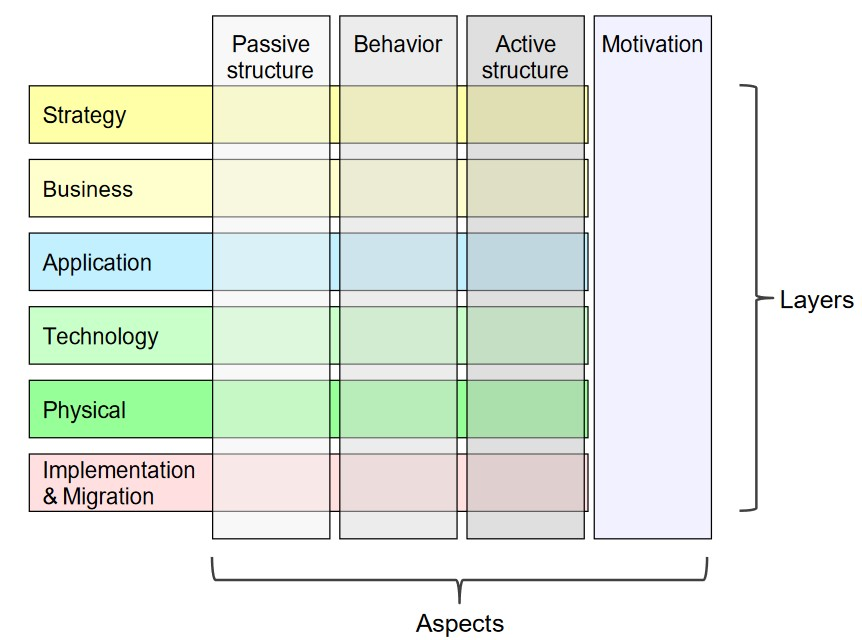
\includegraphics[width=0.7\linewidth]{imgs/coreFramwork}
	\caption{Marco completo de ArchiMate}
\end{figure}

\section{Conceptos y su notación}
El lenguaje ArchiMate separa los conceptos del lenguaje (es decir, los constituyentes del metamodelo) de su notación. Diferentes grupos de interesados pueden requerir diferentes notaciones para comprender un modelo o una visión de la arquitectura.  A este respecto, los ArchiMatelanguages de lenguajes como el UML o el BPMN, que sólo tienen una notación normalizada. El mecanismo de punto de vista explicado en el Capítulo 14 proporciona los medios para definir tales visualizaciones orientadas a las partes interesadas. Aunque la notación de los conceptos de ArchiMate puede (y debería) ser específica de las partes interesadas, la norma proporciona una notación gráfica común, que puede ser utilizada por los arquitectos y otros que desarrollan modelos ArchiMate. Esta notación está dirigida a un público acostumbrado a las técnicas de modelización técnica existentes, como ERD, UML o BPMN, y por lo tanto se asemeja a ellas. En el resto de este documento, a menos que se indique lo contrario, los símbolos utilizados para representar los conceptos del lenguaje representan la notación estándar de ArchiMate.  Esta notación estándar para la mayoría de los elementos consiste en un cuadro con un icono en la esquina superior derecha. En varios casos, este icono por sí mismo puede también utilizarse como notación alternativa. Esta iconografía estándar debe preferirse siempre que sea posible para que cualquier persona que conozca el lenguaje ArchiMate pueda leer los diagramas producidos en el lenguaje.

\subsection{Meta}

La principal jerarquía de elementos de comportamiento y estructura del lenguaje ArchiMate se presenta en la tabla 3.1. Define estos elementos de forma genérica e independiente de la capa. Nótese que la mayoría de estos elementos (las cajas blancas) son elementos abstractos del metamodelo; es decir, no están instanciados en los modelos sino que sólo sirven para estructurar el metamodelo.  La notación presentada es, por lo tanto, la forma genérica en que se representan las especializaciones de estos elementos (es decir, los elementos de las diferentes capas de la arquitectura). Además de describir  los elementos concretos (los recuadros grises), que pueden utilizarse para modelar la Arquitectura de la Empresa a nivel estratégico.

\newpage
\subsubsection{Elementos de la Estructura}
	\begin{table}[h!]
	\begin{tabular}{| m{7em} | m{7cm} | m{3cm} |}
		\hline
		Concepto & Descripción & Representación \\
		
		\hline
		Motivación
		& 
		Un elemento de motivación representa el contexto o la motivación detrás de la  arquitectura de la empresa
		& 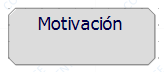
\includegraphics[width=0.8\linewidth, height=0.05\textheight]{imgs/conceptos/meta/Motivacion}
		\\
		
		\hline
		Estructura 
		& 
		Elementos de estructura son equivalentes sinónimos, se subdividen  en estructuras activas ,                              estructuras activas internas,  estructuras activas externas y estructuras pasivas
		& 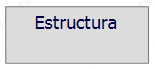
\includegraphics[width=0.8\linewidth, height=0.05\textheight]{imgs/conceptos/meta/Estructura}
		\\
		
		\hline
		Estructura activa  
		& 
		Estructuras que pueden tener un comportamiento
		& 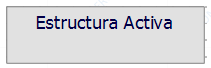
\includegraphics[width=0.8\linewidth, height=0.05\textheight]{imgs/conceptos/meta/EstructuraActiva}
		\\  
		
		\hline
		Estructura activa externa  
		& 
		Llamado interfase representa un punto de acceso donde uno o mas servicios son prestados al ambiente  
		&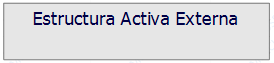
\includegraphics[width=0.8\linewidth, height=0.05\textheight]{imgs/conceptos/meta/EstructuraActivaExterna}
		\\
		
		\hline
		Estructura activa interna
		& 
		Es un elemento que representa una entidad que es capaz de mostrar comportamiento
		& 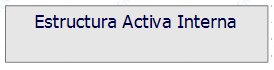
\includegraphics[width=0.8\linewidth, height=0.05\textheight]{imgs/conceptos/meta/EstructuraActivaInterna.PNG}
		\\
		
		\hline
		Estructura pasiva
		& 
		Es un elemento que representa una entidad sobre la cual se realiza un comportamiento
		& 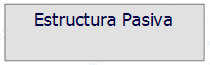
\includegraphics[width=0.8\linewidth, height=0.05\textheight]{imgs/conceptos/meta/EstructuraPasiva.PNG}
		\\
		
		\hline
		Interfase
		& 
		Representa un punto de acceso donde uno o mas servicios son puestos en el ambiente.
		& 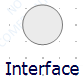
\includegraphics[width=0.8\linewidth, height=0.05\textheight]{imgs/conceptos/meta/Interface.PNG}
		\\
		
		\hline
		
		Comportamiento
		& 
		Es un elemento que equivale a un verbo se  subdivide en evento ,comportamiento interno, proceso , función, interacción, comportamiento externo y servicio.
		& 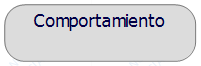
\includegraphics[width=0.8\linewidth, height=0.05\textheight]{imgs/conceptos/meta/Comportamiento.PNG}
		\\
		
		\hline
		Evento
		&
		Representa un cambio de estado 
		& 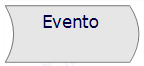
\includegraphics[width=0.8\linewidth, height=0.05\textheight]{imgs/conceptos/meta/Evento.PNG}
		\\
		
		\hline
		Elemento de comportamiento interno 
		& 
		Representa una o mas unidades de actividades que pueden ser realizadas por uno o mas elementos de estructura activa
		& 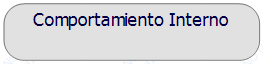
\includegraphics[width=0.8\linewidth, height=0.05\textheight]{imgs/conceptos/meta/ComportamientoInterno.PNG}
		\\	\hline
	\end{tabular}
	%\caption{}
	\label{tab:concepts}
\end{table}

\newpage
\begin{table}[h!]
\begin{center}
	\begin{tabular}{| m{6em} | m{7cm} | m{3cm} |}
		\hline
		Concepto & Descripción & Representación \\ 
		
		\hline
		Servicio
		&
		Un servicio es un comportamiento del sistema proveedor  visible  externamente 
		&
		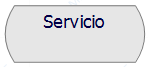
\includegraphics[width=0.8\linewidth, height=0.05\textheight]{imgs/conceptos/meta/Servicio.PNG}
		\\
		
		\hline
		Función
		& 
		Representa una colección de comportamientos, basado en una colección de criterios específicos, tales como fuente requerida, competencias o localización   
		& 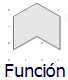
\includegraphics[width=0.8\linewidth, height=0.05\textheight]{imgs/conceptos/meta/Funcion.PNG}
		\\
		
		\hline
		Proceso
		& 
		Representa una secuencia de comportamientos que consiguen un resultado especifico
		& 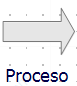
\includegraphics[width=0.8\linewidth, height=0.05\textheight]{imgs/conceptos/meta/Proceso.PNG}
		\\
		
		\hline
		Interacción  
		& 
		Representa una unidad de comportamientos que deben ser realizados por dos o mas elementos de estructura activa interna , ya sea a través de una asignación directa o agregados en una colaboración 
		& 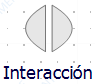
\includegraphics[width=0.8\linewidth, height=0.05\textheight]{imgs/conceptos/meta/Interaccion.PNG}
		\\
		
		\hline
		Colaboración  
		& 
		Representa un acuerdo entre dos o mas elementos estructuras activas internas, trabajan juntos para realizar algún comportamiento colectivo   
		& 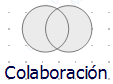
\includegraphics[width=0.8\linewidth, height=0.05\textheight]{imgs/conceptos/meta/Colaboracion.PNG}
		\\
		
		\hline
		Elemento de comportamiento externo
		& 
		Representa un comportamiento explicito que es visible en el exterior  
		& 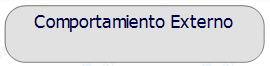
\includegraphics[width=0.8\linewidth, height=0.05\textheight]{imgs/conceptos/meta/ComportamientoExterno.PNG}
		\\
		
		\hline
		
		Elementos compuestos 
		&
		Son elementos que se basan en aspectos de otras capas del lenguaje   
		&
		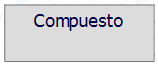
\includegraphics[width=0.8\linewidth, height=0.05\textheight]{imgs/conceptos/meta/Compuesto.PNG}
		\\
		
		\hline
	\end{tabular}
	\caption{Conceptos capa meta}
	\label{tab:concepts}
\end{center}
\end{table}

\section{Punto de Vista de Motivación}
En esta vista de motivación permite diseñar al modelador los elementos de motivación por medio de influenciadores. En esta vista se resume las vistas anteriores dando lugar a tener las caracterizaras mas importantes de la vista motivacional.

\subsection{Modelo de Motivación}
\begin{figure}[h!]
	\centering
	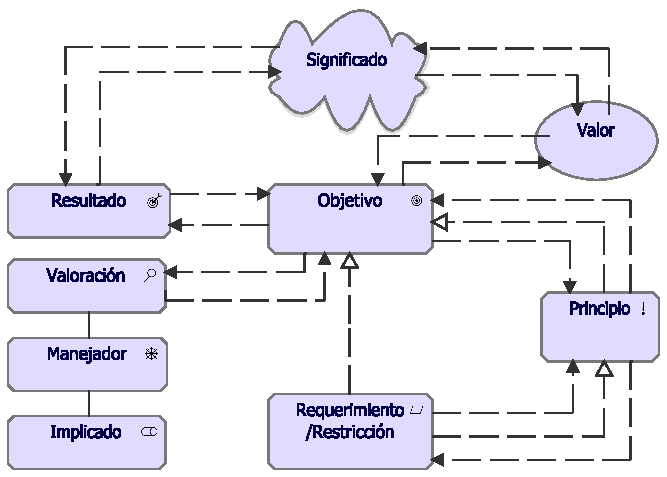
\includegraphics[width=1.0\linewidth]{imgs/modelo/Motivacion}
	\caption{Modelo Motivación}
\end{figure}

Los elementos de motivación se utilizan para modelar las motivaciones, o razones, que guían el diseño o cambio de una arquitectura empresarial. Entre los elementos mas importantes se tiene el implicado: aquel que se implica en el objetivo estudiado, por otro lado tenemos el alcance: aquel que da la motivación, entre otros mas elementos que radican en la motivación e influencia que ejercen sobre los objetivos estratégicos

%\newpage

\subsection{Caso  de Motivación}
\begin{figure}[h!]
	\centering
	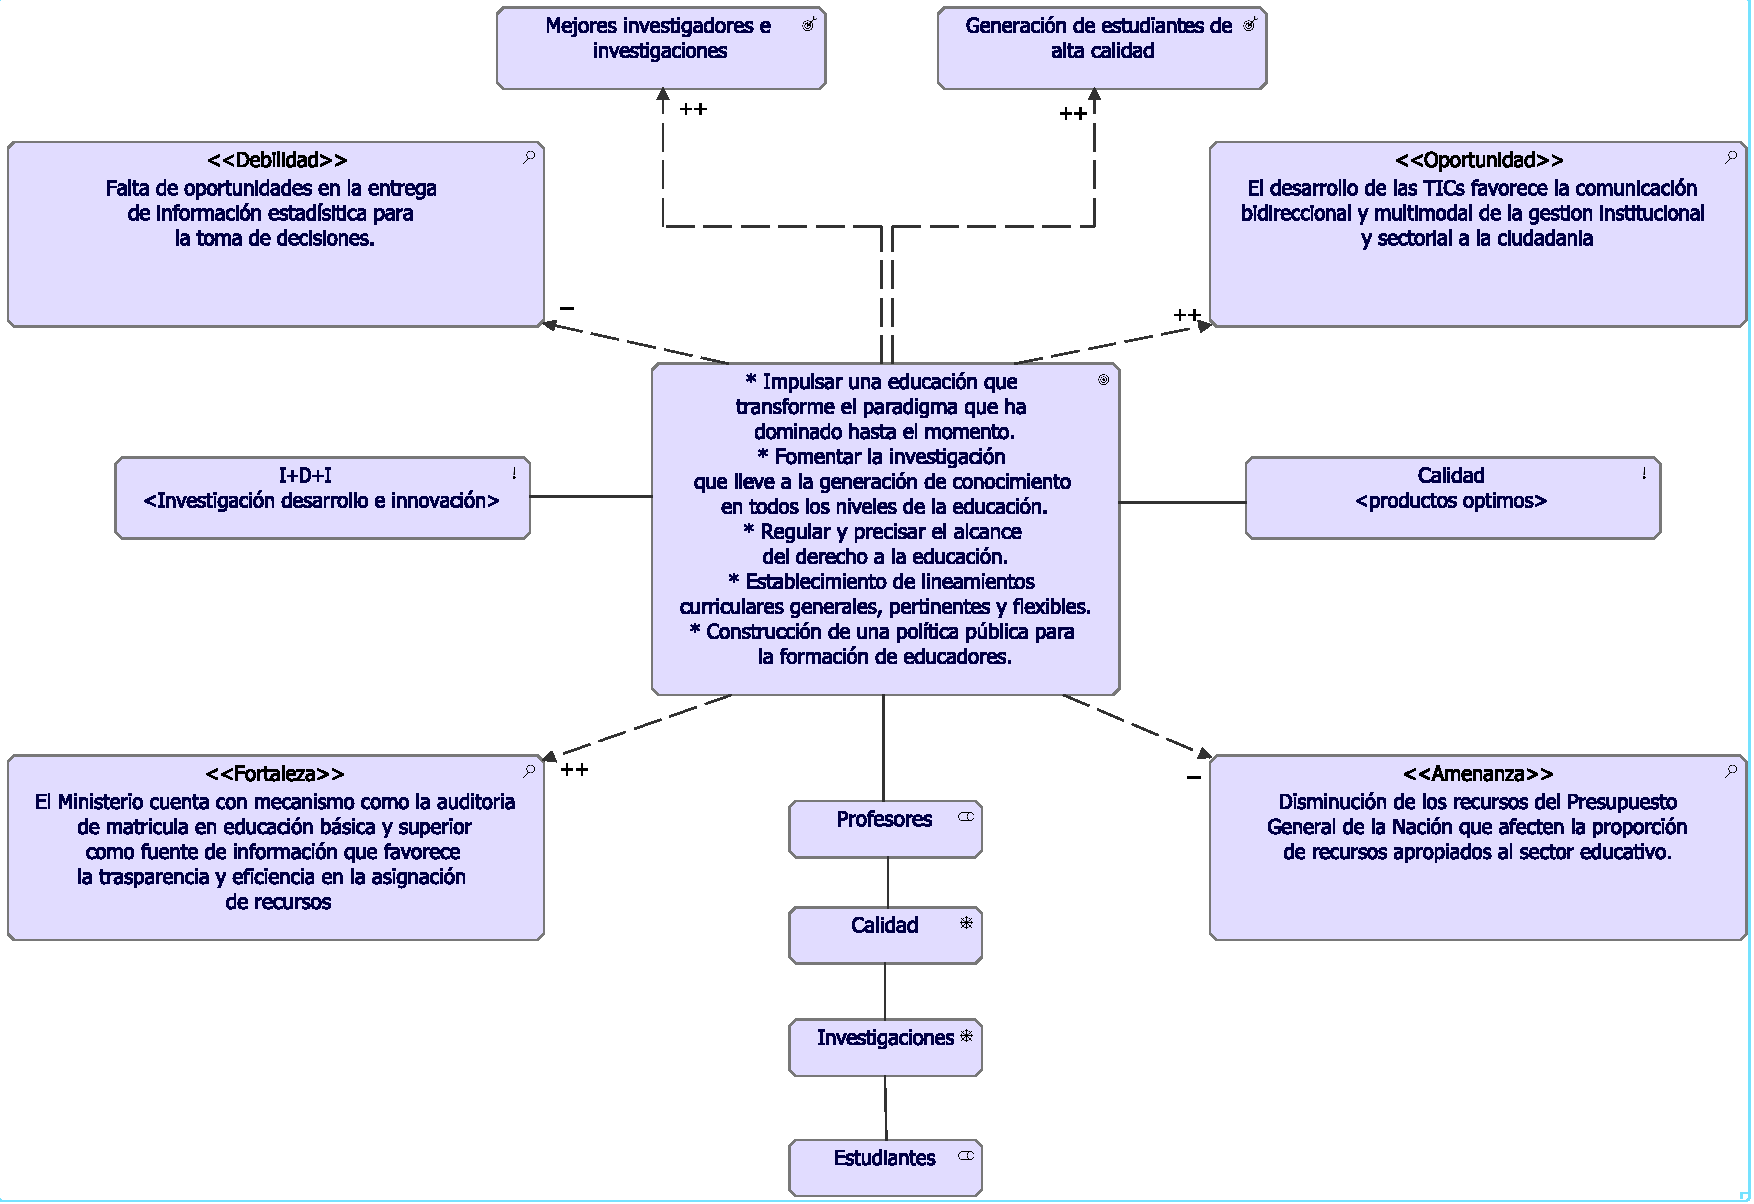
\includegraphics[width=1.0\linewidth]{imgs/motivacion/motivacion/motivacion}
	\caption{Caso Motivación}
\end{figure}

El análisis DOFA es un importante elemento que permite encontrar las estrategias que envuelven objetivos con el fin de mejorar los fines de una empresa. Para los objetivos agrupados en el caso de estudio de motivación tenemos las fortaleza: el ministerio usa la auditoria de la educación para favorecer la eficiencia de los recursos suministrados. La falta de oportunidad para tomar decisiones es una debilidad de la organización. Los implicados que están relacionados con una educación de calidad en este caso de estudio se tienen a los profesores impulsando calidad en sus enseñanzas logrando investigaciones y estudiantes de tal grado.    


\chapter{Estrategia}
\section{Introduccion}
Además de los elementos de motivación descritos en el \ref{chap:Motivacional}, el lenguaje también incluye una serie de elementos de estrategia, en particular la capacidad, los recursos y el curso de acción, como se muestra en la figura 4. Estos se definen como especializaciones de los elementos genéricos de comportamiento y estructura y se definen con más detalle en el capítulo 7.

\newpage

\section{Metamodelo}
\begin{figure}[h!]
	\centering
	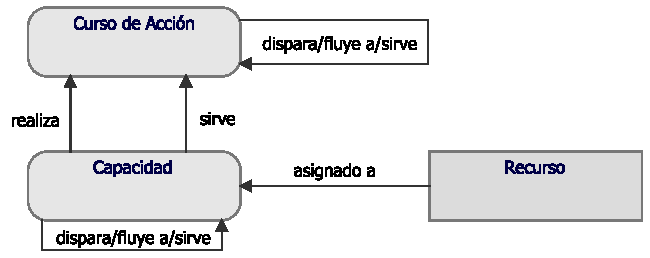
\includegraphics[width=0.9\linewidth]{imgs/meta/Estrategia}
	\caption{Metamodelo Motivacional}
\end{figure}

descripcion....

\newpage
\chapter{Estrategia}
\section{Introduccion}
Además de los elementos de motivación descritos en el \ref{chap:Motivacional}, el lenguaje también incluye una serie de elementos de estrategia, en particular la capacidad, los recursos y el curso de acción, como se muestra en la figura 4. Estos se definen como especializaciones de los elementos genéricos de comportamiento y estructura y se definen con más detalle en el capítulo 7.

\newpage

\section{Metamodelo}
\begin{figure}[h!]
	\centering
	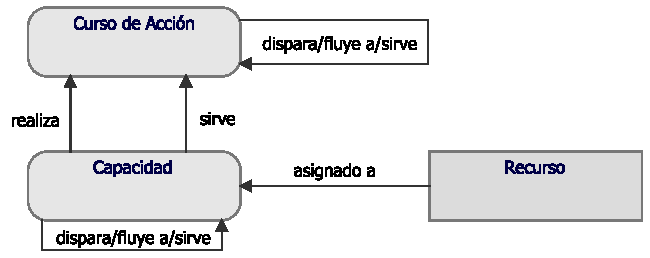
\includegraphics[width=0.9\linewidth]{imgs/meta/Estrategia}
	\caption{Metamodelo Motivacional}
\end{figure}

descripcion....

\newpage
\chapter{Estrategia}
\section{Introduccion}
Además de los elementos de motivación descritos en el \ref{chap:Motivacional}, el lenguaje también incluye una serie de elementos de estrategia, en particular la capacidad, los recursos y el curso de acción, como se muestra en la figura 4. Estos se definen como especializaciones de los elementos genéricos de comportamiento y estructura y se definen con más detalle en el capítulo 7.

\newpage

\section{Metamodelo}
\begin{figure}[h!]
	\centering
	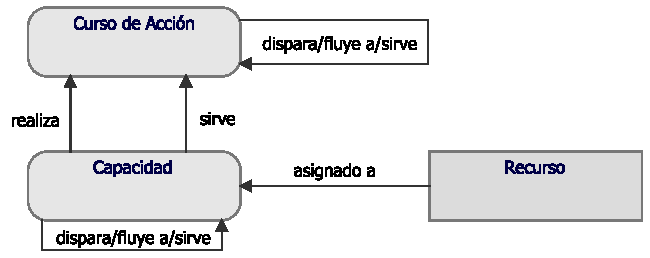
\includegraphics[width=0.9\linewidth]{imgs/meta/Estrategia}
	\caption{Metamodelo Motivacional}
\end{figure}

descripcion....

\newpage
\include{arquitectura/estrategia/estrategia}

\newpage
\include{arquitectura/estrategia/capacidad}


\newpage
\include{arquitectura/estrategia/resultado}

\newpage
\include{arquitectura/estrategia/recurso}



\newpage
\section{Punto de Vista de Mapa de Capacidad}

El punto de vista del mapa de capacidades permite al arquitecto de la empresa crear una visión general estructurada de las capacidades de la empresa. Un mapa de capacidad típicamente muestra dos o tres niveles de capacidades en toda la empresa. Puede, por ejemplo, utilizarse como mapa de calor para identificar áreas de inversión. En algunos casos, un mapa de capacidades también puede mostrar los resultados específicos que ofrecen esas capacidades.

\subsection{Modelo de Mapa de Capacidad}
\begin{figure}[h!]
	\centering
	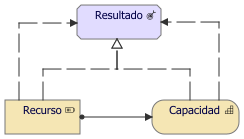
\includegraphics[width=.5\linewidth]{imgs/caso/MapaCapacidad}
	\caption{Modelo Mapa de Capacidad}
\end{figure}

En sínstesis, un recurso es un activo que es propiedad o está controlado por un individuo u organización. Por otra parte, una capacidad es una habilidad que posee un elemento de estructura activa, como una organización, una persona o un sistema. Y, finalmente, un curso de acción es un enfoque o plan para configurar algunas capacidades y recursos de la empresa, dispustos para la consecusión de un objetivo. \\

Aumentar el beneficio es un objetivo que puede descomponerse en varios otros objetivos: Disminuir los costos y aumentar los ingresos. El primero está relacionado con la estrategia de Operación Excelencia de la empresa, modelada como un curso de acción. Estos resultan en dos resultados: Disminución de los costos y pérdida de clientes, que influyen en los objetivos de manera positiva y negativa. Esto muestra una importante diferencia entre los objetivos y los resultados: no todos los resultados conducen a los resultados previstos.
Los cursos de acción se realizan por una serie de capacidades: Gestión y operaciones de TI y gestión de productos, y los recursos apropiados Recursos humanos y recursos de TI se asignan a las primeras.

\newpage

\subsection{Caso de Mapa de Capacidad}

\subsubsection{Resutlado 1: Mejores Investigadores e Investigaciones}

\begin{figure}[h!]
	\centering
	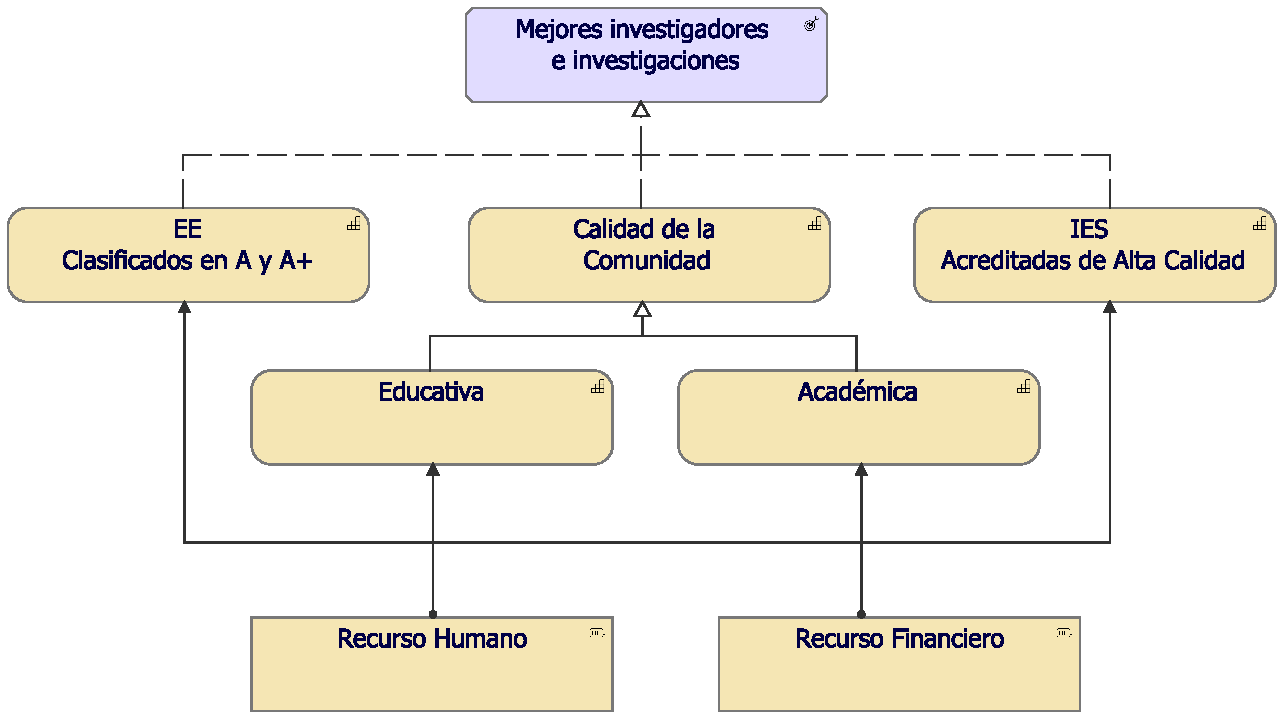
\includegraphics[width=1\linewidth]{imgs/modelo/estrategia/capacidad/1.pdf}
	\caption{Caso Mapa de Capacidad}
\end{figure}

Para dar alcance al resultado de obtener mejores investigadores y mejores investigaciones, el MEN como estructura activa se basa en las habilidades inmersas tanto en los Establecimientos Educativos de calificación A y A+ \footnote{\url{https://www.icfes.gov.co/documents/20143/193495/Clasificacion+de+establecimientos+y+sedes+Saber+11.pdf/2f177381-3c38-6b20-f5da-272dba42b412}}, los cuales representan la mayoría de los planteles registrados, así como las habilidades al interior de sus Instituciones de Educación Superior acreditadas de alta calidad. \\

No obstante, estas habilidades se encuentran arraigadas a la capacidad provista por la calidad de la comunidad, educativa y académica respectivamente. A saber, el activo más importante del MEN, el recurso humano; y que, junto al recurso financiero, conforman el punto de partida para el curso de acción de la organización.

\clearpage
\subsubsection{Resutlado 2: Generación de Estudiantes de Alta Calidad}

\begin{figure}[h!]
	\centering
	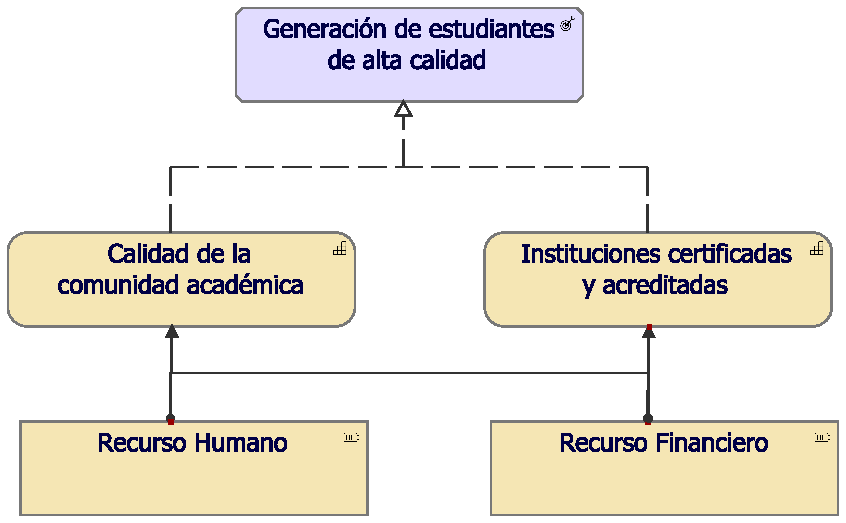
\includegraphics[width=.7\linewidth]{imgs/modelo/estrategia/capacidad/2.pdf}
	\caption{Caso Mapa de Capacidad}
\end{figure}

En en el marco de la \textbf{generación de estudiantes} de alta calidad, el MEN dispone de dos capacidades como lo son la calidad de la comunidad académica e instituciones certificadas y acreditadas que garantizan el desarrollo de procesos con altos estándares de calidad. Las cuales, junto con los recursos humano y financiero, se encuntran configurados dentro del curso de acción para la consecusión de dicho objetivo.


\newpage
\section{Punto de Vista de Realización de resultado}

El punto de vista de la realización de resultados se utiliza para mostrar cómo las capacidades y los elementos básicos subyacentes producen resultados de más alto nivel orientados al negocio.

\subsection{Modelo de Realización de resultado}
\begin{figure}[h!]
	\centering
	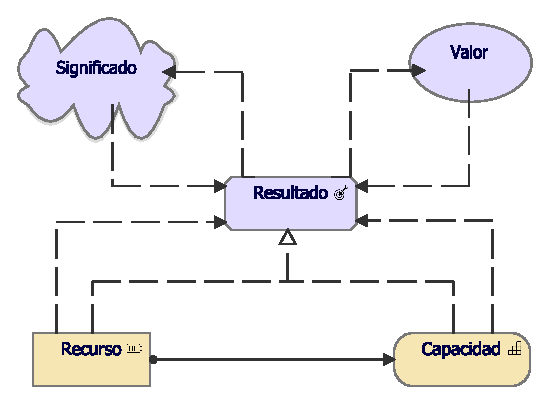
\includegraphics[width=.5\linewidth]{imgs/caso/RealResultado.pdf}
	\caption{Modelo Realización de resultado}
\end{figure}

El punto de vista de la realización de resultados describe cómo las capacidades y los recursos de la empresa producen resultados de alto nivel orientados al negocio.

\newpage

\subsection{Caso de Realización de resultado}

\subsubsection{Resultado 1: Mejores Investigadores e Investigaciones}

\begin{figure}[h!]
	\centering
	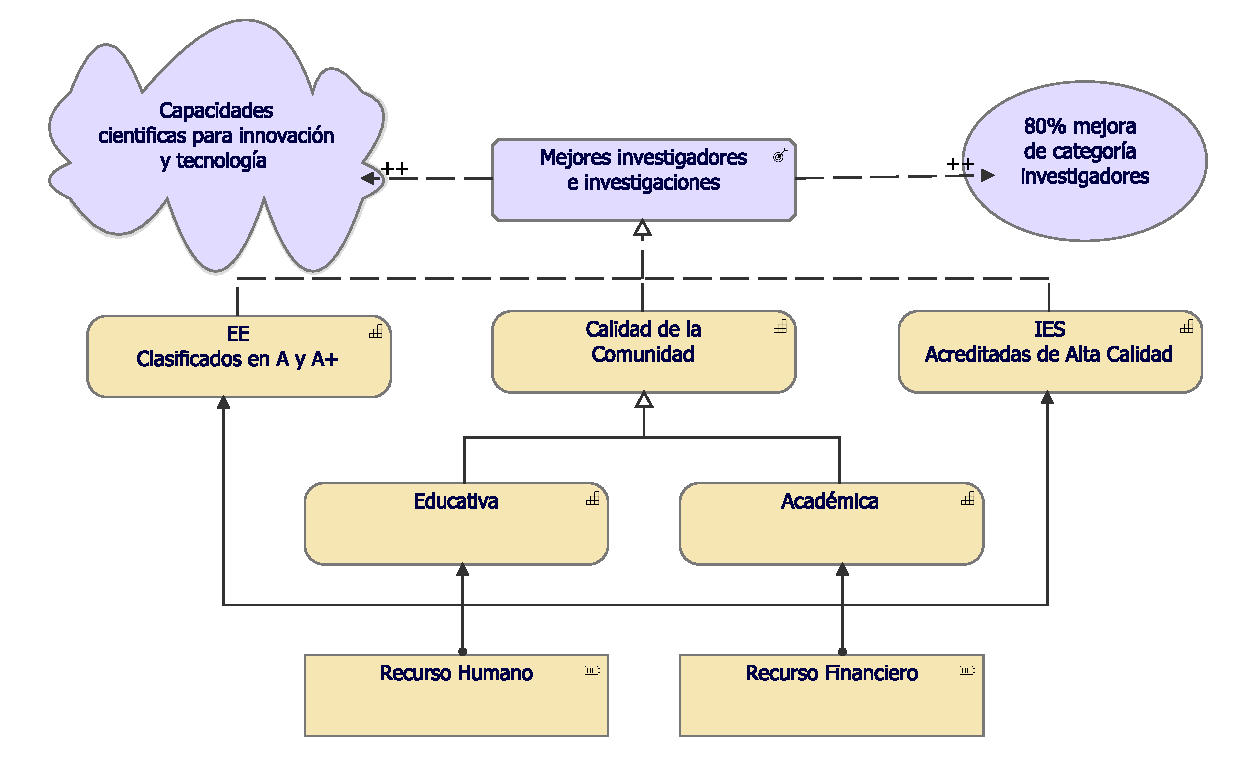
\includegraphics[width=.8\linewidth]{imgs/modelo/estrategia/resultado/resultado_2.pdf}
	\caption{Caso Realización de resultado}
\end{figure}

Para el caso de resultado de \textbf{Mejores Investigadores e Investigaciones} se busca promover nuevas capacidades científicas que fomenten la innovación y la tecnología gracias comunidad de calidad, de las IES acreditadas de alta calidad. Se pretende alcanzar el 80 por ciento en subir de categoría por parte de los investigadores.


\clearpage
\subsubsection{Resultado 2: Generación de Estudiantes de Alta Calidad}

\begin{figure}[h!]
	\centering
	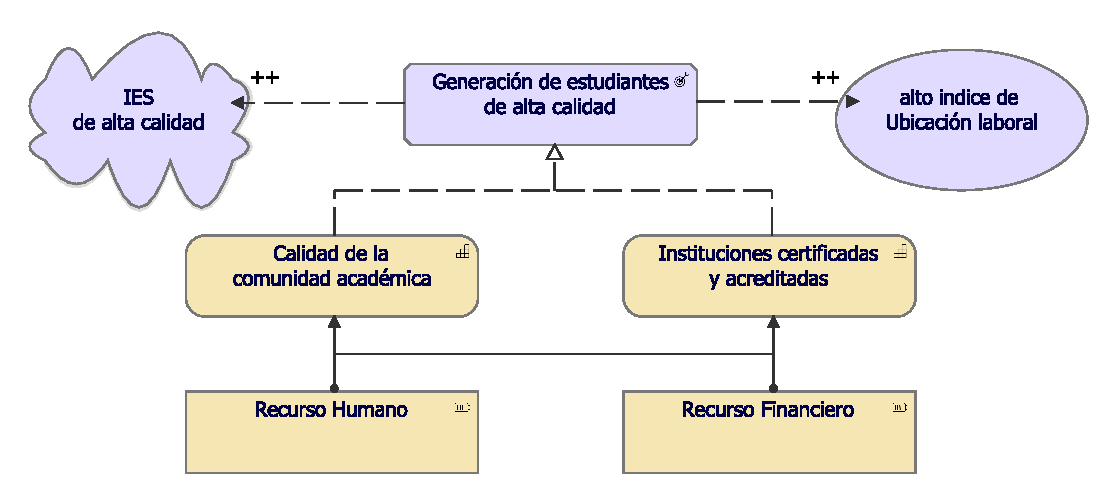
\includegraphics[width=.8\linewidth]{imgs/modelo/estrategia/resultado/resultado.pdf}
	\caption{Caso Realización de resultado}
\end{figure}

El resultado de \textbf{generación de estudiantes de alta calidad} proporciona un significado de grandes expectativas para el MEN, puesto que este resultado da como garantía Instituciones de Educación Superior(IES) de alta calidad promoviendo la capacidad de calidad en la comunidad académica ademas de instituciones certificadas y acreditadas.

\newpage
\section{Punto de Vista de Mapa de Recurso}

El punto de vista del mapa de recursos permite al arquitecto comercial crear una descripción general estructurada de los recursos de la empresa. Un mapa de recursos generalmente muestra dos o tres niveles de recursos en toda la empresa. Puede, por ejemplo, utilizarse como mapa de calor para identificar áreas de inversión. En algunos casos, un mapa de recursos también puede mostrar relaciones entre los recursos y las capacidades a las que están asignados.

\subsection{Modelo de Mapa de Recurso}
\begin{figure}[h!]
	\centering
	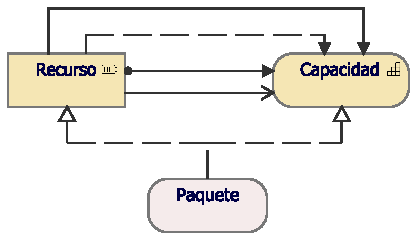
\includegraphics[width=.5\linewidth]{imgs/caso/MapaRecurso.pdf}
	\caption{Modelo Mapa de Recurso}
\end{figure}

El punto de vista del mapa de recursos proporciona una descripción estructurada de los recursos de la empresa.

\newpage

\subsection{Caso de Mapa de Recurso}

\subsubsection{Resultado 1: Mejores Investigadores e Investigaciones}

\begin{figure}[h!]
	\centering
	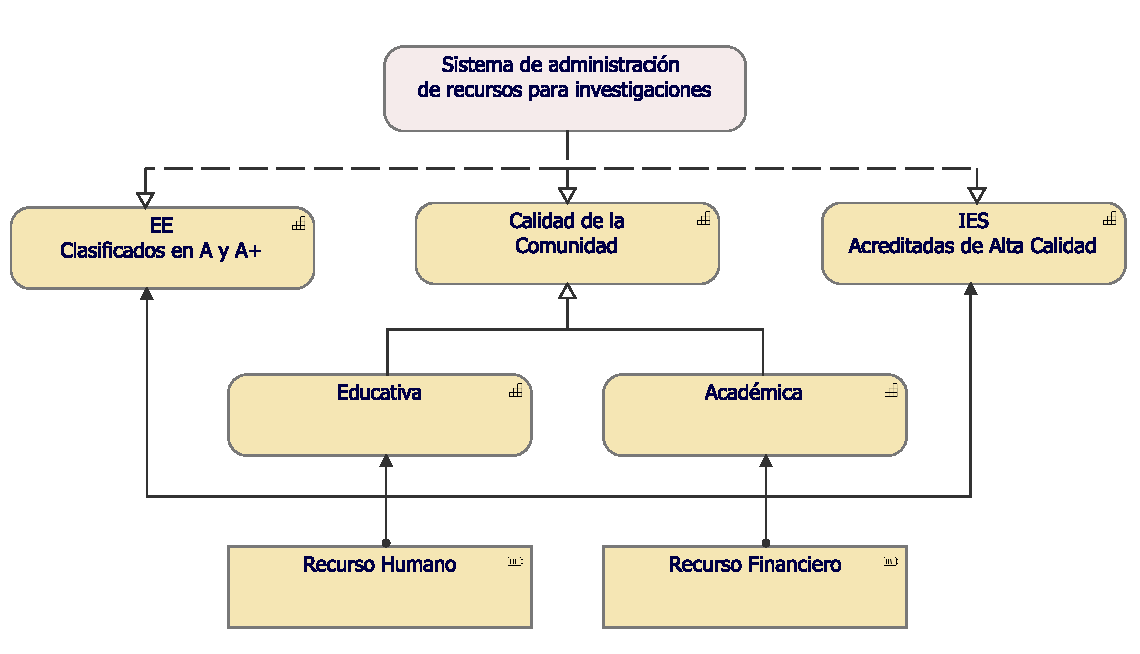
\includegraphics[width=1\linewidth]{imgs/modelo/estrategia/mapa/mapa_recurso.pdf}
	\caption{Caso Mapa de Recurso}
\end{figure}

Para dar alcance a las capacidades de calidad de la comunidad, IES Acreditadas de Alta Calidad y EE Clasificados en A y A+ basadas en habilidades dadas por el resultado de Mejores Investigadores e Investigaciones, se pretende construir un sistema que administre de manera optima los recursos para realizar nuevas investigaciones dando lugar a un crecimiento exponencial de nuevos investigadores.

\clearpage
\subsubsection{Resultado 2: Generación de Estudiantes de Alta Calidad}

\begin{figure}[h!]
	\centering
	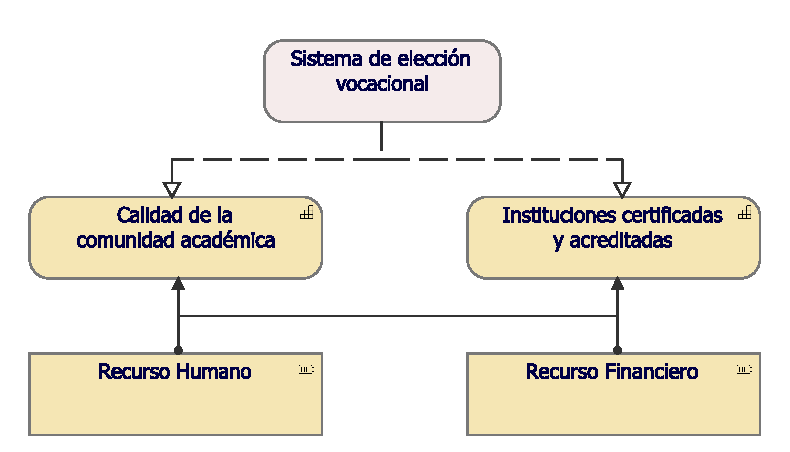
\includegraphics[width=.8\linewidth]{imgs/modelo/estrategia/mapa/mapa_recurso_2.pdf}
	\caption{Caso Mapa de Recurso}
\end{figure}

Para garantizar la generación de estudiantes de calidad es necesario implantar nuevos sistemas que ayudan a elegir de mejor manera la vocación que tendrán en el futuro los estudiantes. Buscando así que el estudiante se acerque a las diferentes carreras o áreas del conocimiento sin sentir presión por parte de ningún ente, que aquella vocación escogida por el estudiante sea totalmente de su agrado y gusto; formando estudiantes que lleven la educación de calidad no por obligación sino por interés propio.



\newpage
\section{Punto de Vista de Mapa de Capacidad}

El punto de vista del mapa de capacidades permite al arquitecto de la empresa crear una visión general estructurada de las capacidades de la empresa. Un mapa de capacidad típicamente muestra dos o tres niveles de capacidades en toda la empresa. Puede, por ejemplo, utilizarse como mapa de calor para identificar áreas de inversión. En algunos casos, un mapa de capacidades también puede mostrar los resultados específicos que ofrecen esas capacidades.

\subsection{Modelo de Mapa de Capacidad}
\begin{figure}[h!]
	\centering
	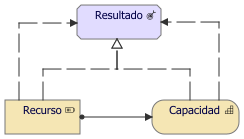
\includegraphics[width=.5\linewidth]{imgs/caso/MapaCapacidad}
	\caption{Modelo Mapa de Capacidad}
\end{figure}

En sínstesis, un recurso es un activo que es propiedad o está controlado por un individuo u organización. Por otra parte, una capacidad es una habilidad que posee un elemento de estructura activa, como una organización, una persona o un sistema. Y, finalmente, un curso de acción es un enfoque o plan para configurar algunas capacidades y recursos de la empresa, dispustos para la consecusión de un objetivo. \\

Aumentar el beneficio es un objetivo que puede descomponerse en varios otros objetivos: Disminuir los costos y aumentar los ingresos. El primero está relacionado con la estrategia de Operación Excelencia de la empresa, modelada como un curso de acción. Estos resultan en dos resultados: Disminución de los costos y pérdida de clientes, que influyen en los objetivos de manera positiva y negativa. Esto muestra una importante diferencia entre los objetivos y los resultados: no todos los resultados conducen a los resultados previstos.
Los cursos de acción se realizan por una serie de capacidades: Gestión y operaciones de TI y gestión de productos, y los recursos apropiados Recursos humanos y recursos de TI se asignan a las primeras.

\newpage

\subsection{Caso de Mapa de Capacidad}

\subsubsection{Resutlado 1: Mejores Investigadores e Investigaciones}

\begin{figure}[h!]
	\centering
	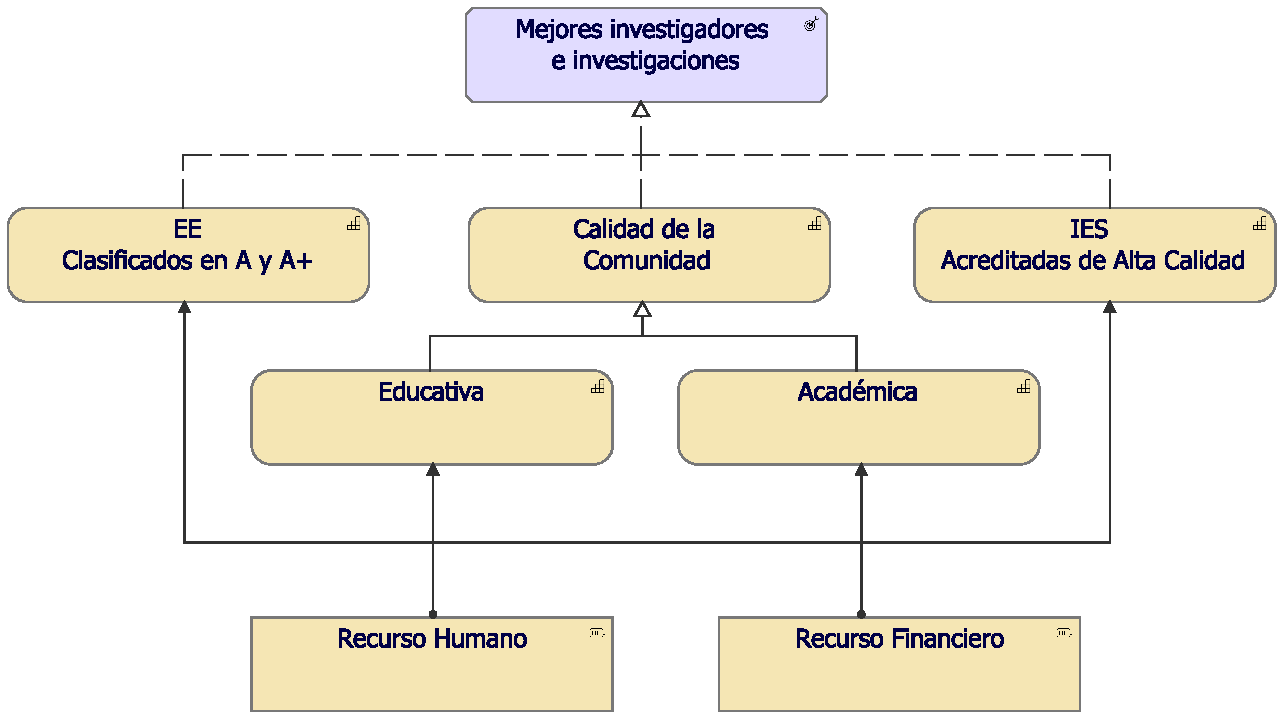
\includegraphics[width=1\linewidth]{imgs/modelo/estrategia/capacidad/1.pdf}
	\caption{Caso Mapa de Capacidad}
\end{figure}

Para dar alcance al resultado de obtener mejores investigadores y mejores investigaciones, el MEN como estructura activa se basa en las habilidades inmersas tanto en los Establecimientos Educativos de calificación A y A+ \footnote{\url{https://www.icfes.gov.co/documents/20143/193495/Clasificacion+de+establecimientos+y+sedes+Saber+11.pdf/2f177381-3c38-6b20-f5da-272dba42b412}}, los cuales representan la mayoría de los planteles registrados, así como las habilidades al interior de sus Instituciones de Educación Superior acreditadas de alta calidad. \\

No obstante, estas habilidades se encuentran arraigadas a la capacidad provista por la calidad de la comunidad, educativa y académica respectivamente. A saber, el activo más importante del MEN, el recurso humano; y que, junto al recurso financiero, conforman el punto de partida para el curso de acción de la organización.

\clearpage
\subsubsection{Resutlado 2: Generación de Estudiantes de Alta Calidad}

\begin{figure}[h!]
	\centering
	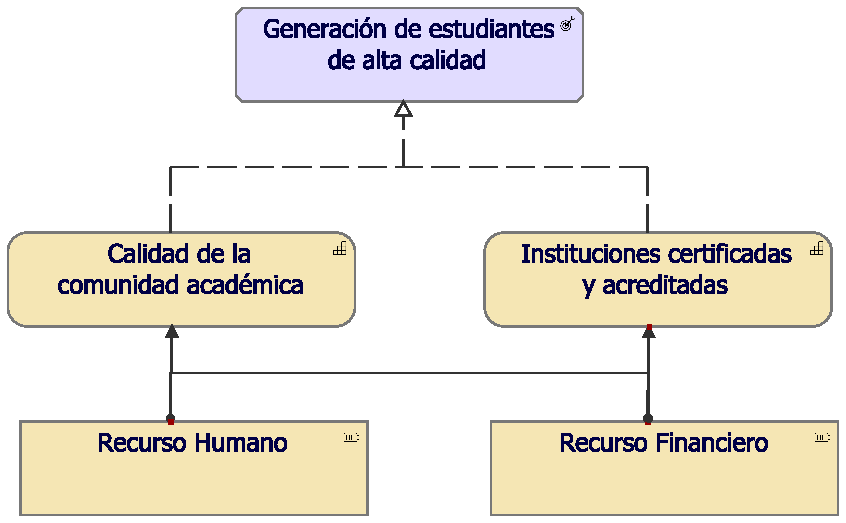
\includegraphics[width=.7\linewidth]{imgs/modelo/estrategia/capacidad/2.pdf}
	\caption{Caso Mapa de Capacidad}
\end{figure}

En en el marco de la \textbf{generación de estudiantes} de alta calidad, el MEN dispone de dos capacidades como lo son la calidad de la comunidad académica e instituciones certificadas y acreditadas que garantizan el desarrollo de procesos con altos estándares de calidad. Las cuales, junto con los recursos humano y financiero, se encuntran configurados dentro del curso de acción para la consecusión de dicho objetivo.


\newpage
\section{Punto de Vista de Realización de resultado}

El punto de vista de la realización de resultados se utiliza para mostrar cómo las capacidades y los elementos básicos subyacentes producen resultados de más alto nivel orientados al negocio.

\subsection{Modelo de Realización de resultado}
\begin{figure}[h!]
	\centering
	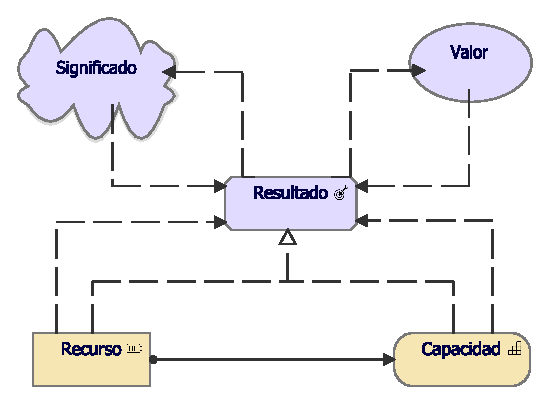
\includegraphics[width=.5\linewidth]{imgs/caso/RealResultado.pdf}
	\caption{Modelo Realización de resultado}
\end{figure}

El punto de vista de la realización de resultados describe cómo las capacidades y los recursos de la empresa producen resultados de alto nivel orientados al negocio.

\newpage

\subsection{Caso de Realización de resultado}

\subsubsection{Resultado 1: Mejores Investigadores e Investigaciones}

\begin{figure}[h!]
	\centering
	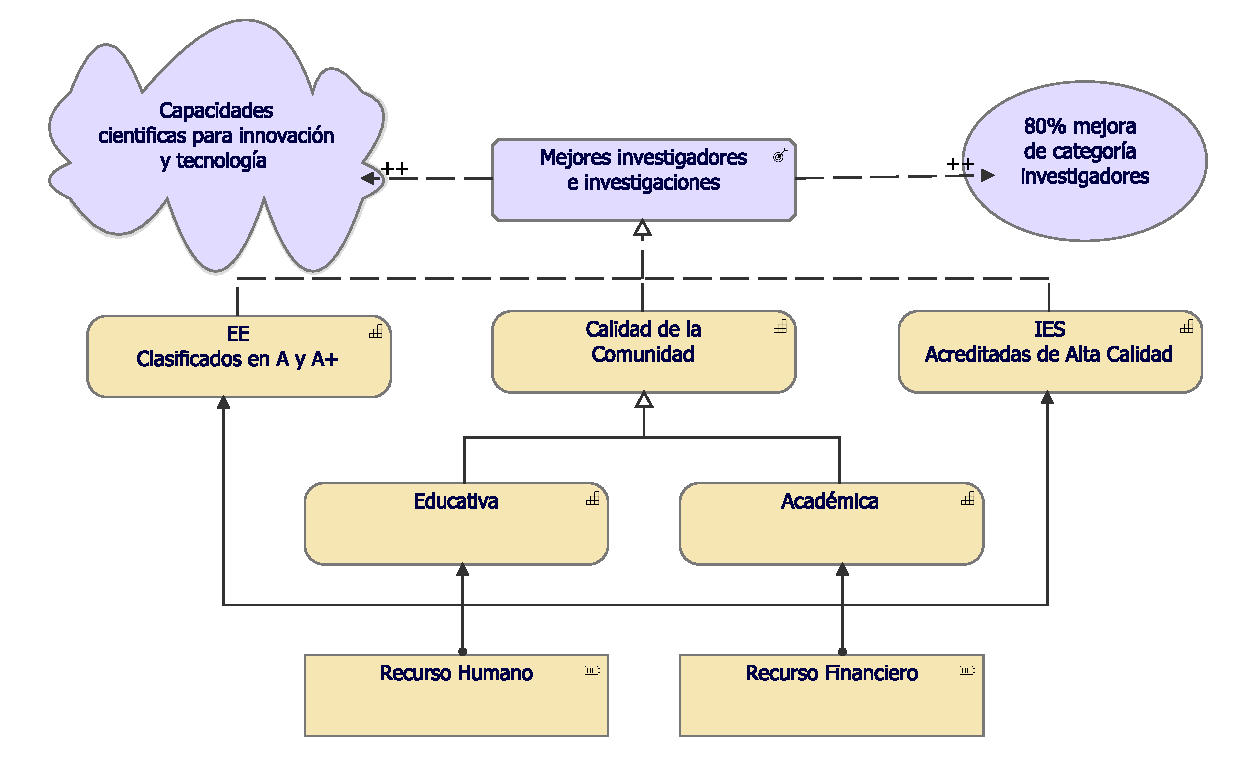
\includegraphics[width=.8\linewidth]{imgs/modelo/estrategia/resultado/resultado_2.pdf}
	\caption{Caso Realización de resultado}
\end{figure}

Para el caso de resultado de \textbf{Mejores Investigadores e Investigaciones} se busca promover nuevas capacidades científicas que fomenten la innovación y la tecnología gracias comunidad de calidad, de las IES acreditadas de alta calidad. Se pretende alcanzar el 80 por ciento en subir de categoría por parte de los investigadores.


\clearpage
\subsubsection{Resultado 2: Generación de Estudiantes de Alta Calidad}

\begin{figure}[h!]
	\centering
	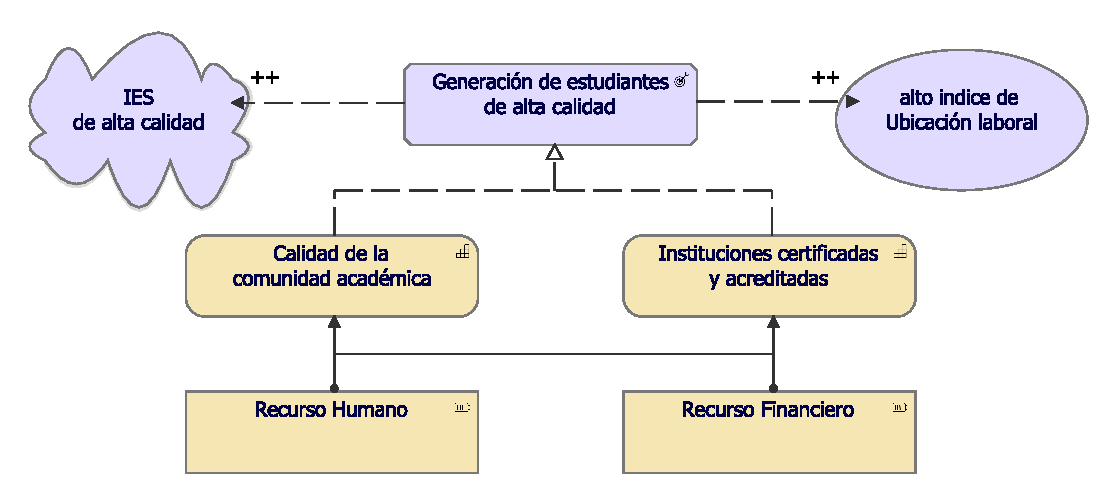
\includegraphics[width=.8\linewidth]{imgs/modelo/estrategia/resultado/resultado.pdf}
	\caption{Caso Realización de resultado}
\end{figure}

El resultado de \textbf{generación de estudiantes de alta calidad} proporciona un significado de grandes expectativas para el MEN, puesto que este resultado da como garantía Instituciones de Educación Superior(IES) de alta calidad promoviendo la capacidad de calidad en la comunidad académica ademas de instituciones certificadas y acreditadas.

\newpage
\section{Punto de Vista de Mapa de Recurso}

El punto de vista del mapa de recursos permite al arquitecto comercial crear una descripción general estructurada de los recursos de la empresa. Un mapa de recursos generalmente muestra dos o tres niveles de recursos en toda la empresa. Puede, por ejemplo, utilizarse como mapa de calor para identificar áreas de inversión. En algunos casos, un mapa de recursos también puede mostrar relaciones entre los recursos y las capacidades a las que están asignados.

\subsection{Modelo de Mapa de Recurso}
\begin{figure}[h!]
	\centering
	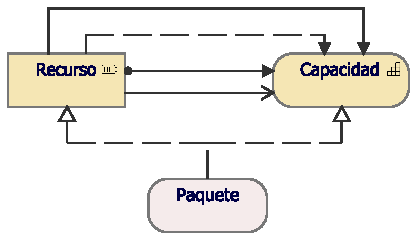
\includegraphics[width=.5\linewidth]{imgs/caso/MapaRecurso.pdf}
	\caption{Modelo Mapa de Recurso}
\end{figure}

El punto de vista del mapa de recursos proporciona una descripción estructurada de los recursos de la empresa.

\newpage

\subsection{Caso de Mapa de Recurso}

\subsubsection{Resultado 1: Mejores Investigadores e Investigaciones}

\begin{figure}[h!]
	\centering
	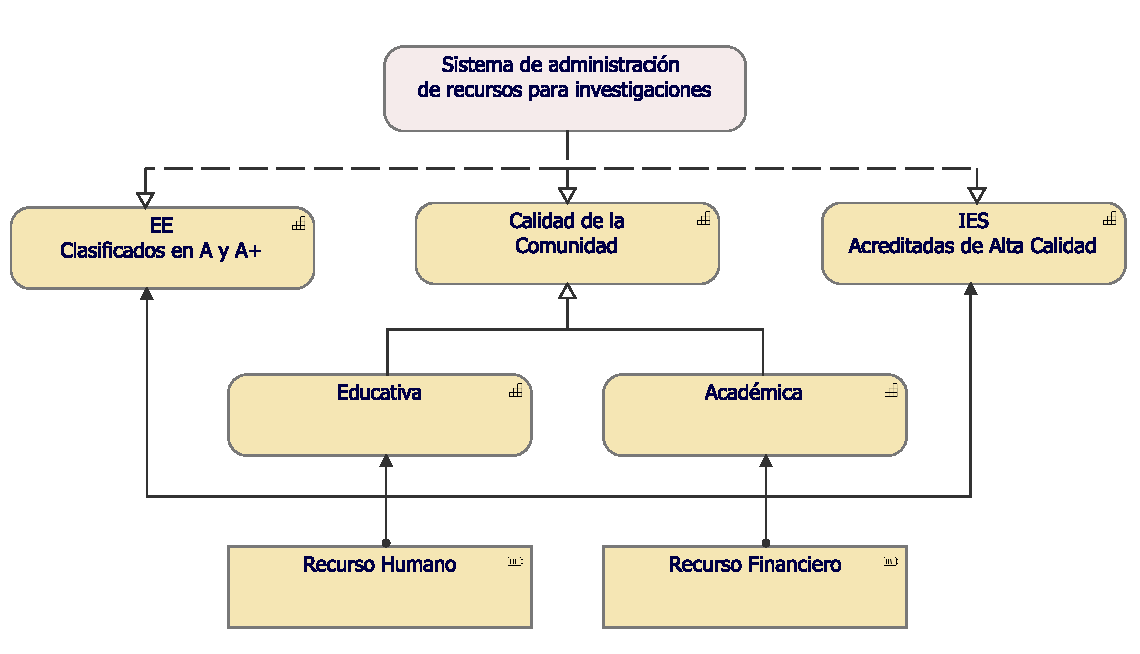
\includegraphics[width=1\linewidth]{imgs/modelo/estrategia/mapa/mapa_recurso.pdf}
	\caption{Caso Mapa de Recurso}
\end{figure}

Para dar alcance a las capacidades de calidad de la comunidad, IES Acreditadas de Alta Calidad y EE Clasificados en A y A+ basadas en habilidades dadas por el resultado de Mejores Investigadores e Investigaciones, se pretende construir un sistema que administre de manera optima los recursos para realizar nuevas investigaciones dando lugar a un crecimiento exponencial de nuevos investigadores.

\clearpage
\subsubsection{Resultado 2: Generación de Estudiantes de Alta Calidad}

\begin{figure}[h!]
	\centering
	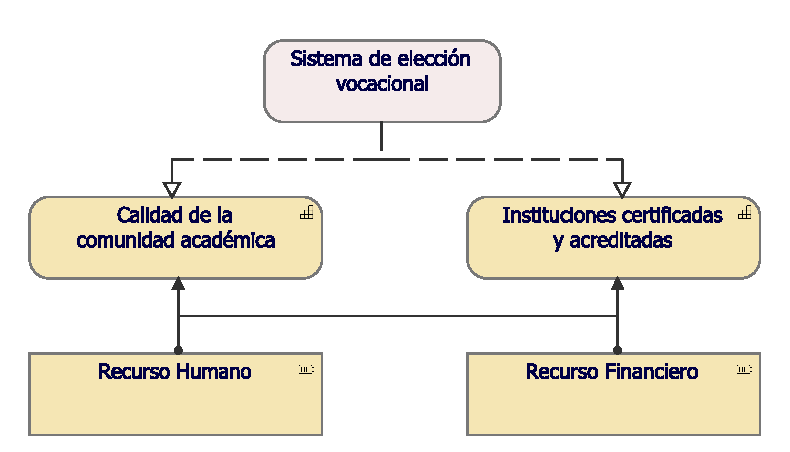
\includegraphics[width=.8\linewidth]{imgs/modelo/estrategia/mapa/mapa_recurso_2.pdf}
	\caption{Caso Mapa de Recurso}
\end{figure}

Para garantizar la generación de estudiantes de calidad es necesario implantar nuevos sistemas que ayudan a elegir de mejor manera la vocación que tendrán en el futuro los estudiantes. Buscando así que el estudiante se acerque a las diferentes carreras o áreas del conocimiento sin sentir presión por parte de ningún ente, que aquella vocación escogida por el estudiante sea totalmente de su agrado y gusto; formando estudiantes que lleven la educación de calidad no por obligación sino por interés propio.



\chapter{Negocio}
\section{Introducción}
Las descripciones arquitectónicas se centran en la estructura, lo que significa que las interrelaciones de las entidades dentro de una organización desempeñan un papel importante. Para hacerlo explícito, se ha introducido el elemento de la colaboración empresarial.\\

Se introduce el elemento de la interfaz empresarial para modelar explícitamente los lugares o canales (lógicos o físicos) en los que se puede acceder a los servicios que una función ofrece al entorno. El mismo servicio puede ofrecerse en varias interfaces diferentes; por ejemplo, por correo, por teléfono o a través de Internet. A diferencia de la modelización de aplicaciones, en los enfoques actuales de modelización de la capa empresarial no es frecuente reconocer el elemento de interfaz empresarial.
En la Capa de Negocio se definen tres tipos de elementos de estructura activa interna: actor comercial, papel comercial y colaboración comercial.\\

El aspecto de la estructura pasiva de la Capa de Negocios contiene los elementos de estructura pasiva (objetos de negocios) que son manipulados por el comportamiento, como los procesos o funciones de negocios. Las entidades pasivas representan los conceptos importantes en los que la empresa piensa en un dominio.
En la Capa de Negocios, hay dos tipos principales de elementos de estructura pasiva: objeto de negocio y representación. Además, un contrato, utilizado en el contexto de un producto, es una especialización de un objeto de negocio.

\newpage
\section{Metamodelo}

\begin{figure}[h!]
	\centering
	\begin{minipage}{1\textwidth} % choose width suitably
	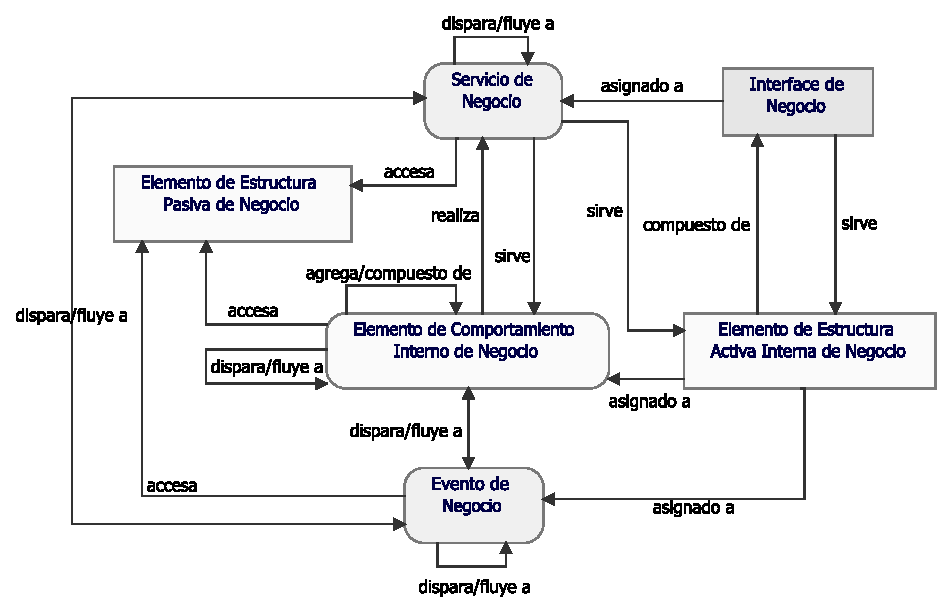
\includegraphics[width=0.9\linewidth]{imgs/meta/Negocio}
	\caption{Metamodelo Negocio}
	\label{fig:business}
	{\footnotesize Nota: Esta figura no muestra todas las relaciones permitidas; cada elemento del lenguaje puede tener relaciones de composición, agregación y especialización con elementos del mismo tipo; además, hay relaciones indirectas que pueden derivarse.\par}
	\end{minipage}
\end{figure}

La figura \ref{fig:business} ofrece una visión general de los elementos de la capa de negocios y sus relaciones. El elemento de estructura activa interna de la empresa, el elemento de comportamiento interno de la empresa y el elemento de estructura pasiva de la empresa son elementos abstractos; sólo sus especializaciones (como se definen en las siguientes secciones) se instancian en los modelos.

La Capa de Negocios se utiliza típicamente (a menudo en conjunto con los elementos de estrategia descritos en el Capítulo 5) para modelar la arquitectura de negocios de una empresa, definida por el marco del TOGAF como una descripción de la estructura e interacción entre la estrategia de negocios, la organización, las funciones, los procesos de negocios y las necesidades de información.

\newpage
\section{Punto de Vista de Organización}

El punto de vista de la organización se centra en la organización (interna) de una empresa, un departamento, una red de empresas o de otra entidad organizativa. Es posible presentar modelos en este punto de vista como diagramas de bloques anidados, pero también de una manera más tradicional, como los organigramas. El punto de vista de la organización es muy útil para identificar las competencias, la autoridad y las responsabilidades de una organización.

\subsection{Modelo de Organización}
\begin{figure}[h!]
	\centering
	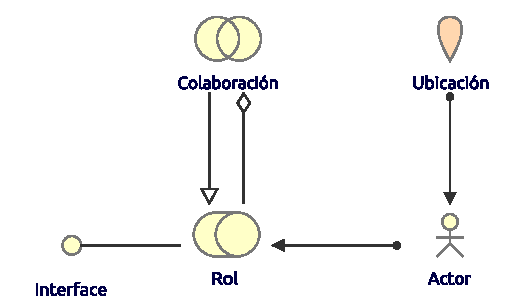
\includegraphics[width=.6\linewidth]{imgs/modelo/Organizacion}
	\caption{Modelo Organizacion}
\end{figure}

Un actor de negocios es una entidad de negocios que es capaz de realizar un comportamiento. Los actores pueden incluir entidades fuera de la organización real; por ejemplo, clientes y socios. Un actor comercial puede representar a esas entidades comerciales en diferentes niveles de detalle, y puede corresponder tanto a un actor como a una unidad organizativa en el marco del TOGAF. Ejemplos de actores comerciales son los seres humanos, los departamentos y las unidades comerciales. Una colaboración empresarial es un conjunto de dos o más elementos de la estructura activa interna de la empresa que trabajan juntos para llevar a cabo un comportamiento colectivo. Una interfaz de negocios es un punto de acceso en el que se pone a disposición del entorno un servicio comercial. Una interfaz comercial expone la funcionalidad de un servicio comercial a otros roles o actores comerciales. Se suele denominar canal (teléfono, Internet, oficina local, etc.). El mismo servicio comercial puede estar expuesto a través de diferentes interfaces.

\newpage
\subsection{Caso  de Organización}
\begin{figure}[h!]
	\centering
	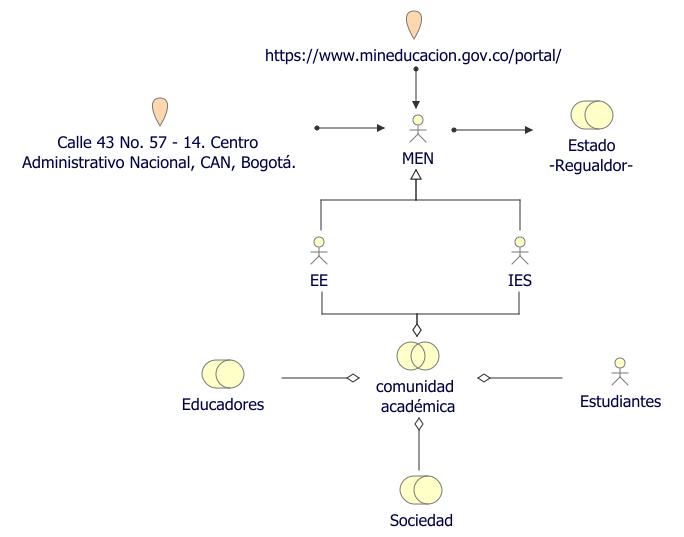
\includegraphics[width=.9\linewidth]{imgs/caso/negocio/organizacion}
	\caption{Caso Organizacion}
\end{figure}

El MEN tiene como actores principales los establecimientos educativos (EE), las instituciones de educación superior (IES) y las comunidades estudiantiles respectivas. Además, cuenta con ubicaciones tanto física como virtual, a saber, dispone de una dirección electrónica de dominio gubernamental como lo es \url{https://www.mineducacion.gov.co/portal/} y de una dirección física ubicada en la calle 43 No. 57 - 14 Centro 
Administrativo Nacional, CAN, Bogotá. Por otra parte, encontramos tres roles a destacar siendo el Estado uno de ellos y ejerciendo como ente regulador de las políticas a majear, así como, de emisor de recursos económicos junto con otro rol como lo es la sociedad y que, a su vez esta sociedad junto con el último de los roles a destacar, los educadores, colaboran o confluyen en una comunidad académica junto con los estudiantes, como otro de los actores principales de la organización.



\clearpage
\section{Punto de Vista de Cooperación de Actor}


\subsection{Modelo de Cooperación de Actor}
\begin{figure}[h!]
	\centering
	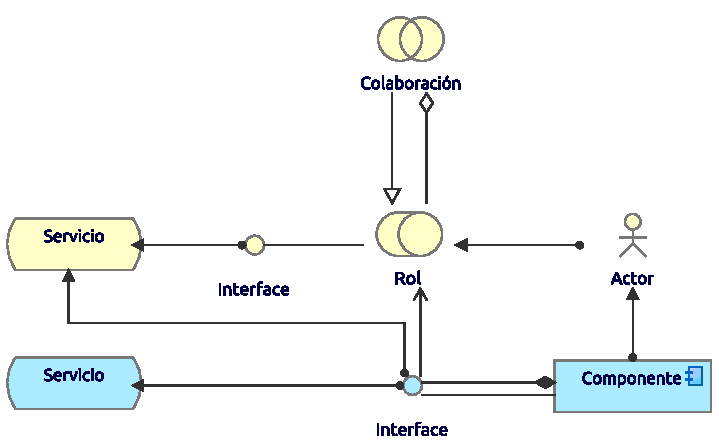
\includegraphics[width=.6\linewidth]{imgs/modelo/CoopActor.pdf}
	\caption{Modelo Cooperacion de Actor}
\end{figure}

El punto de vista de cooperación de actor establece las colaboraciones que existen internamente y externamente sobre un actor o rol de la organización con el fin de mostrar de qué manera interactuan e interfiere con el actor en cuestión. Por medio de interfaces  que comunican los entes del exterior y el interior de la organización con el actor o rol.

\newpage
\subsection{Caso  de Cooperación de Actor}
\begin{figure}[h!]
	\centering
	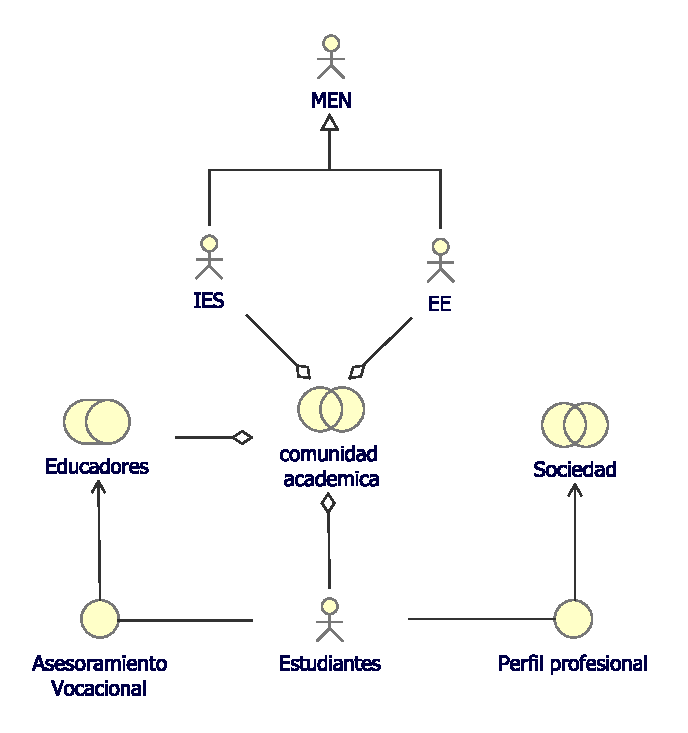
\includegraphics[width=.8\linewidth]{imgs/caso/negocio/coperacion_actor.pdf}
	\caption{Caso Cooperacion de Actor}
\end{figure}

Para nuestro objeto de estudio en relación al punto de vista de colaboración de actor tenemos como actor principal a los estudiantes aquellos que colaboran en la comunidad académica y hacen parte de las IES y EE que son regidas por el Ministerio de Educación. Por otro lado tenemos el rol de educador que hace parte de la comunidad y que puede ayudar a guiar en parte la vocación que construirá en un futuro el estudiante. Los estudiantes contribuirán en la sociedad gracias a su perfil que se ha formado durante sus años de estudio y que permitirán a las empresas apoderarse de estos individuos y así lograr mejores avances que colaboren en su entidad y por tanto a la sociedad misma.

\clearpage
\section{Punto de Vista de función de Negocio}

El punto de vista de la cooperación de los procesos comerciales se utiliza para mostrar las relaciones de uno o más procesos comerciales entre sí y/o con su entorno. Puede utilizarse tanto para crear un diseño de alto nivel de los procesos empresariales dentro de su contexto como para proporcionar a un director operacional responsable de uno o más de esos procesos una visión de sus dependencias. Los aspectos importantes de la cooperación en los procesos empresariales son:

\begin{itemize}
	\item Relaciones causales entre los principales procesos comerciales de la empresa
	\item Mapeo de los procesos comerciales en las funciones comerciales
	\item Realización de servicios por procesos comerciales
	\item Uso de datos compartidos
\end{itemize}

Cada una de ellas puede considerarse un "subpunto de vista" del punto de vista de la cooperación en los procesos comerciales.

\subsection{Modelo de función de Negocio}
\begin{figure}[h!]
	\centering
	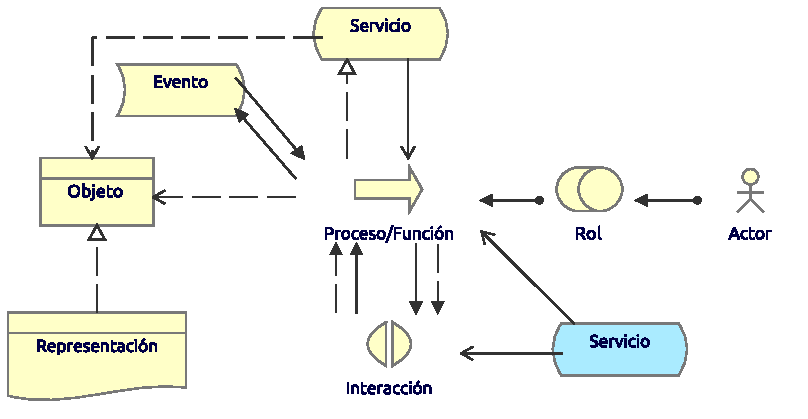
\includegraphics[width=.8\linewidth]{imgs/modelo/ProcesoNegocio}
	\caption{Modelo función de Negocio}
\end{figure}

Un proceso empresarial representa una secuencia de comportamientos empresariales que logra un resultado específico, como un conjunto definido de productos o servicios empresariales.
Un proceso de negocios describe el comportamiento interno realizado por un rol de negocios que se requiere para producir un conjunto de productos y servicios. Para un consumidor, los productos y servicios son relevantes y el comportamiento requerido es meramente una caja negra, de ahí la designación "interno".
Un proceso comercial complejo puede ser una agregación de otros procesos de grano más fino. A cada uno de ellos se le pueden asignar funciones más finas.
Existe una relación potencial de muchos a muchos entre los procesos de negocios y las funciones de negocios. En términos informales, los procesos describen algún tipo de "flujo" de actividades, mientras que las funciones agrupan las actividades según las aptitudes, los conocimientos, los recursos, etc. requeridos. Un proceso empresarial puede ser desencadenado por, o desencadenar, cualquier otro elemento de comportamiento empresarial (por ejemplo, un acto empresarial, un proceso empresarial, una función empresarial o una interacción empresarial). Un proceso empresarial puede acceder a objetos empresariales. Un proceso empresarial puede realizar uno o más servicios empresariales y pueden utilizar servicios comerciales (internos) o servicios de aplicación. Se puede asignar una función empresarial a un proceso empresarial para realizar este proceso manualmente. Un proceso empresarial automatizado puede realizarse mediante un proceso de aplicación. El nombre de un proceso empresarial debe indicar claramente una secuencia predefinida de acciones, y puede incluir la palabra "proceso". Ejemplos de ello son "adjudicar la reclamación", "incorporación de empleados", "proceso de aprobación" o "presentación de informes financieros". \\

Un objeto comercial representa un concepto utilizado dentro de un dominio comercial determinado. Un contrato representa una especificación formal o informal de un acuerdo entre un proveedor y un consumidor en el que se especifican los derechos y obligaciones asociados a un producto y se establecen parámetros funcionales y no funcionales para la interacción. Una representación representa una forma perceptible de la información que lleva un objeto comercial.

\clearpage
\subsection{Caso  de función de Negocio}
\begin{figure}[h!]
	\centering
	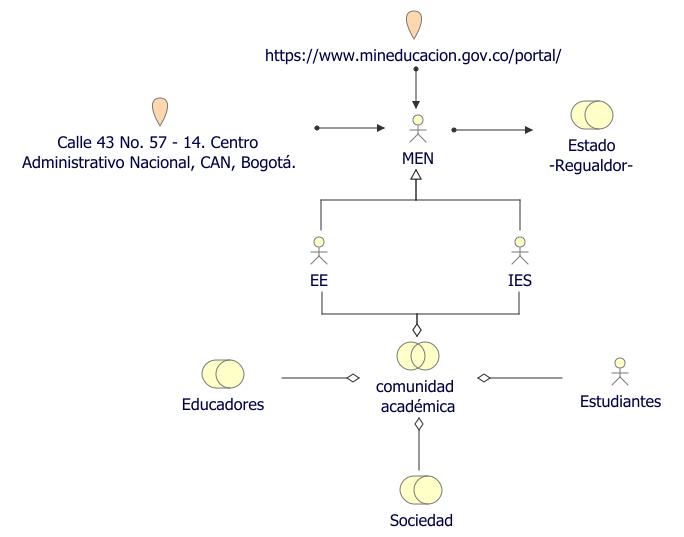
\includegraphics[width=.9\linewidth]{imgs/caso/negocio/organizacion}
	\caption{Caso función de Negocio}
\end{figure}
descripcion...


\clearpage
\section{Punto de Vista de Proceso de Negocio}

El punto de vista de la cooperación de los procesos comerciales se utiliza para mostrar las relaciones de uno o más procesos comerciales entre sí y/o con su entorno. Puede utilizarse tanto para crear un diseño de alto nivel de los procesos empresariales dentro de su contexto como para proporcionar a un director operacional responsable de uno o más de esos procesos una visión de sus dependencias. Los aspectos importantes de la cooperación en los procesos empresariales son:

\begin{itemize}
	\item Relaciones causales entre los principales procesos comerciales de la empresa
	\item Mapeo de los procesos comerciales en las funciones comerciales
	\item Realización de servicios por procesos comerciales
	\item Uso de datos compartidos
\end{itemize}

Cada una de ellas puede considerarse un "subpunto de vista" del punto de vista de la cooperación en los procesos comerciales.

\subsection{Modelo de Proceso de Negocio}
\begin{figure}[h!]
	\centering
	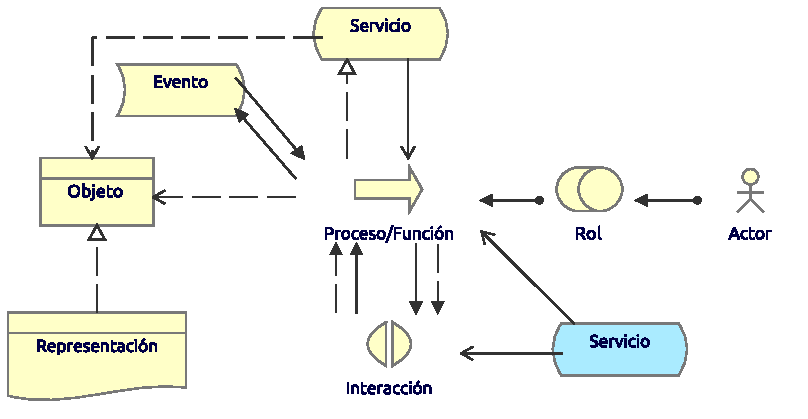
\includegraphics[width=.8\linewidth]{imgs/modelo/ProcesoNegocio}
	\caption{Modelo Proceso de Negocio}
\end{figure}

Un proceso empresarial representa una secuencia de comportamientos empresariales que logra un resultado específico, como un conjunto definido de productos o servicios empresariales.
Un proceso de negocios describe el comportamiento interno realizado por un rol de negocios que se requiere para producir un conjunto de productos y servicios. Para un consumidor, los productos y servicios son relevantes y el comportamiento requerido es meramente una caja negra, de ahí la designación "interno".
Un proceso comercial complejo puede ser una agregación de otros procesos de grano más fino. A cada uno de ellos se le pueden asignar funciones más finas.
Existe una relación potencial de muchos a muchos entre los procesos de negocios y las funciones de negocios. En términos informales, los procesos describen algún tipo de "flujo" de actividades, mientras que las funciones agrupan las actividades según las aptitudes, los conocimientos, los recursos, etc. requeridos. Un proceso empresarial puede ser desencadenado por, o desencadenar, cualquier otro elemento de comportamiento empresarial (por ejemplo, un acto empresarial, un proceso empresarial, una función empresarial o una interacción empresarial). Un proceso empresarial puede acceder a objetos empresariales. Un proceso empresarial puede realizar uno o más servicios empresariales y pueden utilizar servicios comerciales (internos) o servicios de aplicación. Se puede asignar una función empresarial a un proceso empresarial para realizar este proceso manualmente. Un proceso empresarial automatizado puede realizarse mediante un proceso de aplicación. El nombre de un proceso empresarial debe indicar claramente una secuencia predefinida de acciones, y puede incluir la palabra "proceso". Ejemplos de ello son "adjudicar la reclamación", "incorporación de empleados", "proceso de aprobación" o "presentación de informes financieros". \\

Un objeto comercial representa un concepto utilizado dentro de un dominio comercial determinado. Un contrato representa una especificación formal o informal de un acuerdo entre un proveedor y un consumidor en el que se especifican los derechos y obligaciones asociados a un producto y se establecen parámetros funcionales y no funcionales para la interacción. Una representación representa una forma perceptible de la información que lleva un objeto comercial.

\clearpage
\subsection{Caso  de Proceso de Negocio}
\begin{figure}[h!]
	\centering
	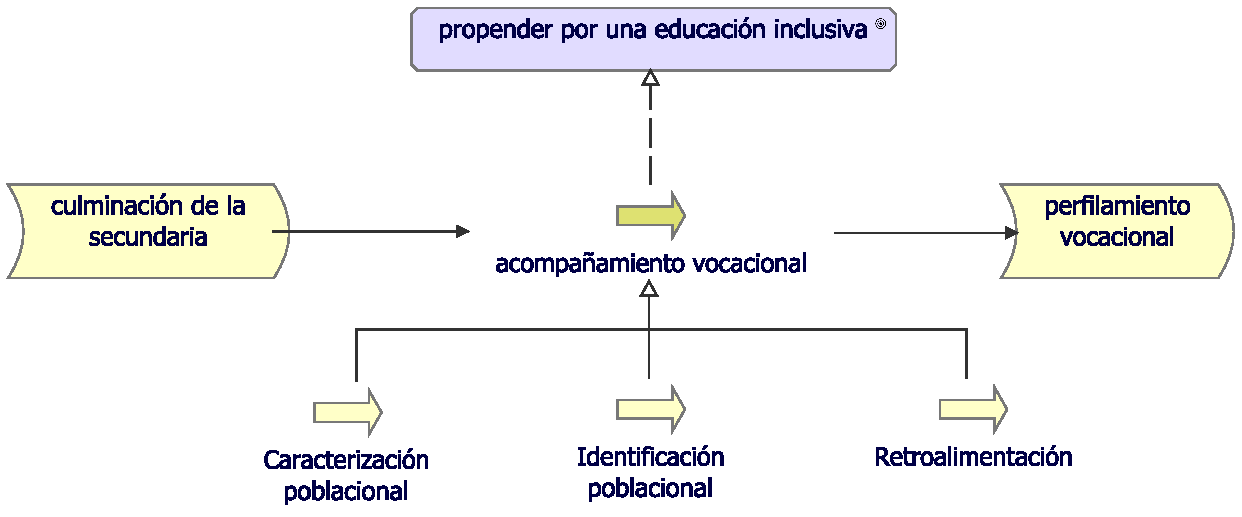
\includegraphics[width=.9\linewidth]{imgs/caso/negocio/proceso}
	\caption{Caso Proceso de Negocio}
\end{figure}

Después de efectuar una revisión documental sobre los procesos del MEN dispuestos para dar alcance a uno de sus principales objetivos, propender por una educación inclusiva, desde nuestra organización proponemos la inclusión de un nuevo proceso capaz de fortalecer y afianzar en la sociedad, ese objetivo de carácter político que conlleve a una educación inclusiva eficiente en cuanto al desarrollo personal y profesional de la comunidad se refiere. Asimismo, este proceso novedoso en el marco actual de la organización, se especializa en tres procesos de carácter secuencial dispuestos de la siguiente manera, una caracterización poblacional, una Identificación poblacional posterior, y finalmente, una retroalimentación individualizada para cada estudiante que culmina la secundaria, evento inicial de nuestro proceso de acompañamiento vocacional, el cual culmina con el perfilamiento vocacional de cada uno de estos estudiantes.



\clearpage
\section{Punto de Vista de Cooperación de Proceso de Negocio}

El punto de vista de cooperación de proceso de negocio, promueve la identificación y asociación de roles a través de procesos, en otras palabras, es la vinculación existente entre los procesos y los roles, este punto de vista se deriva directamente del punto de vista de proceso de negocio y al identificar estos roles, permite expandir la forma en que se entiende el proyecto, asignando responsables a procesos.

\subsection{Modelo de Cooperación de Proceso de Negocio}
\begin{figure}[h!]
	\centering
	\includegraphics[width=.8\linewidth]{imgs/modelo/ProcesoNegocio}
	\caption{Modelo Cooperación de Proceso de Negocio}
\end{figure}

El modelo del punto de vista de Cooperación de Proceso de Negocio, se compone de un conjunto de partes, principalmente mencionadas en la parte exclusiva del proceso de negocio como lo son: el proceso o función, el evento, los derivados de este evento y proceso como el servicio, el objeto, la interacción y la representación y sin dejar de lado el enlace principal con el proceso el cual es el objetivo, estas partes componen tanto al punto de vista de proceso de negocio como al punto de vista de cooperación de proceso de negocio, a excepción que este segundo punto de vista incluye uno o varios roles, el cual se le asigna al proceso en cuestión.

\clearpage
\subsection{Caso de Cooperación de Proceso de Negocio}
\begin{figure}[h!]
	\centering
	\includegraphics[width=.9\linewidth]{imgs/caso/negocio/CoopProNegocio}
	\caption{Caso Cooperación de Proceso de Negocio}
\end{figure}

Este proyecto de colaboración con el Ministerio de Educación Nacional para tener una educación inclusiva y contribuir con el mejoramiento de la educación en el territorio nacional, posee un gran objetivo el cual es el propender por una educación inclusiva, del cual se deriva el proceso principal de tener un acompañamiento vocacional que lo antecede el evento de negocio de la culminación de la secundaria y lo precede el evento del perfilamiento vocacional, a este gran proceso se le asignan dos roles que intervienen en el, como lo son: la secretaría de educación y la población estudiantil además, este proceso principal cuenta con tres sub procesos: la caracterización poblacional, la identificación vocacional que está vinculada con el rol de los profesionales en ciencias humanas y el subproceso de la retroalimentación.



\clearpage
\section{Punto de Vista de Producto}


\subsection{Modelo de Producto}
\begin{figure}[h!]
	\centering
	\includegraphics[width=.6\linewidth]{imgs/modelo/Producto.pdf}
	\caption{Modelo Producto}
\end{figure}

El punto de vista de producto permite ver el conjunto de contratos que rigen un producto de la organización, además relaciona los servicios que se desprenden del producto. Estos contratos son aquello que regulan y limitan  al producto. Los servicios asociados al producto son parte de los objetivos, misión y visión de la empresa y que desembocan en proceso de la organización ya sea implícito o explícito relacionado obviamente con el producto.

\newpage
\subsection{Caso  de Producto}
\begin{figure}[h!]
	\centering
	\includegraphics[width=.9\linewidth]{imgs/caso/negocio/producto.pdf}
	\caption{Caso Producto}
\end{figure}

Para el caso de estudio tenemos como producto de negocio a Tu-Perfil aquel apartado que servirá como guiá para acompañar y perfilar a los estudiantes en la elección de vocación que sera tomada al graduarse como bachiller con el fin de dar cabida al proceso de acompañamiento vocacional que surge de los objetivos de la organización para este caso el MEN.  Este producto esta regido por los contratos definidos ICFES y Titulo de Bachiller, que serán aquellos que limitaran al producto.


\subsection{Aplicación}

Siempre que sea aplicable, la inspiración ha sido tomada de la analogía con la Capa de Negocios. La capa de aplicación se utiliza típicamente para modelar las arquitecturas de los sistemas de información de la empresa, incluida la arquitectura de aplicación que, como se define en el marco del TOGAF, describe la estructura y la interacción de las aplicaciones.

\newpage
\subsubsection{Elementos de la Estructura}
\begin{longtable}{|c|c|c|}
	
	\hline
	Concepto & Descripción & Representación \\ \hline
	
	Componente 
	&
	\begin{tabular}[l]{@{}l@{}}
		Una encapsulación de la funcionalidad\\
		de la aplicación alineada con la \\
		estructura de implementación, que es\\
		modular y reemplazable. Encapsula su\\
		comportamiento y datos, expone los \\
		servicios y los pone a disposición a \\
		través de interfaces.
	\end{tabular}
	& \includegraphics{imgs/aplicacion/componente.pdf}
	\\\hline
	
	Colaboración
	& 
	\begin{tabular}[l]{@{}l@{}}
		Un agregado de dos o más componentes\\
		de la aplicación que trabajan juntos\\
		para realizar un comportamiento de \\
		aplicación colectivo.
	\end{tabular}
	& \includegraphics{imgs/aplicacion/colaboracion.pdf}
	\\\hline
	
	Interface
	& 
	\begin{tabular}[l]{@{}l@{}}
		Un punto de acceso donde los servicios\\
		de la aplicación están disponibles para\\
		un usuario, otro componente de la \\
		aplicación o un nodo.
	\end{tabular}
	& \includegraphics{imgs/aplicacion/interface.pdf}
	\\\hline
	
	Función
	& 
	\begin{tabular}[l]{@{}l@{}}
		Comportamiento automatizado que puede\\
		realizar un componente de la aplicación.
	\end{tabular}
	& \includegraphics{imgs/aplicacion/funcion.pdf}
	\\\hline
	
	Interacción
	& 
	\begin{tabular}[l]{@{}l@{}}
		Una unidad de comportamiento de \\
		aplicación colectiva realizada por \\
		(una colaboración de) dos o más \\
		componentes de la aplicación.
	\end{tabular}
	& \includegraphics{imgs/aplicacion/intereaccion.pdf}
	\\\hline
	
	Proceso
	& 
	\begin{tabular}[l]{@{}l@{}}
		Una secuencia de comportamientos de\\
		aplicación que logra un resultado\\
		específico.
	\end{tabular}
	& \includegraphics{imgs/aplicacion/proceso.pdf}
	\\\hline
	
	Evento 
	& 
	\begin{tabular}[l]{@{}l@{}}
		Un elemento de comportamiento de la\\
		aplicación que denota un cambio de\\
		estado.
	\end{tabular}
	& \includegraphics{imgs/aplicacion/evento.pdf}
	\\\hline
	
	Servicio 
	& 
	\begin{tabular}[l]{@{}l@{}}
		Un comportamiento de aplicación \\
		expuesto definido explícitamente.
	\end{tabular}
	& \includegraphics{imgs/aplicacion/servicio.pdf}
	\\\hline
	
	Objeto
	& 
	\begin{tabular}[l]{@{}l@{}}
		Datos estructurados para \\
		procesamiento automatizado.
	\end{tabular}
	& \includegraphics{imgs/aplicacion/objeto.pdf}
	
	
	\\\hline
	\caption{Conceptos: Aplicaciones}
	\label{tab:concepts}
\end{longtable}

\chapter{Tecnologia}
\section{Introduccion}
contenido...

\newpage

\section{Metamodelo}
\begin{figure}[h!]
	\centering
	\includegraphics[width=0.9\linewidth]{imgs/meta/Tecnologia}
	\caption{Metamodelo Tecnologia}
\end{figure}

descripcion....

\newpage

\section{Punto de Vista de Implementacion y Despliegue}
contenido....
\subsection{Modelo de Implementacion y Despliegue}
\begin{figure}[h!]
	\centering
	\includegraphics[width=.5\linewidth]{imgs/modelo/Implementacion}
	\caption{Modelo Implementacion y Despliegue}
\end{figure}
descripcion...

\newpage

\subsection{Caso  de Implementacion y Despliegue}
\begin{figure}[h!]
	\centering
	\includegraphics[width=.5\linewidth]{imgs/caso/Implementacion}
	\caption{Caso Implementacion y Despliegue}
\end{figure}
descripcion...

\newpage

\subsection{Físico}

Estos se basan en la Capa de Tecnología. No se definen elementos de comportamiento físico separados.  Más bien, los elementos de comportamiento de la Capa de Tecnología (función de la tecnología, proceso, interacción, servicio y evento) se usan para modelar el comportamiento de todos los nodos, incluyendo el equipo físico. Dado que el equipo muy a menudo estará controlado por computadora o tendrá una estrecha relación con la tecnología de la información (piense también en los sensores, Internet de las cosas), su comportamiento puede describirse de manera integral utilizando los conceptos de comportamiento de la tecnología existente.

\newpage
\subsubsection{Elementos de la Estructura}

\begin{longtable}{|c| c| c|}
	\hline
	Concepto & Descripción & Representación \\ \hline
	Facilidad
	&
	\begin{tabular}{p{6cm}p{3cm}}
		Representa un recurso físico que tiene la capacidad de
		facilitar (por ejemplo, albergar o ubicar) el uso de equipos. Por lo general, se utiliza para modelar fábricas, edificios o construcciones al aire libre
	\end{tabular} 
	& \includegraphics[width=0.1\linewidth, height=0.05\textheight]{imgs/conceptos/fisico/facilidad}
	\\
	\hline 
	Equipo
	& 
	\begin{tabular}{p{6cm}p{3cm}}
		El equipo comprende todos los elementos de procesamiento activos que llevan a cabo procesos físicos en los que se utilizan o transforman materiales.
	\end{tabular} 
	& \includegraphics[width=0.1\linewidth, height=0.05\textheight]{imgs/conceptos/fisico/equipo}
	\\
	\hline
	Red de distribución
	&
	\begin{tabular}{p{6cm}p{3cm}} 
		Representa la distribución física o la infraestructura de transporte. Encarna la realización física de las rutas lógicas entre nodos. Una red de distribución conecta dos o más nodos. Una red de distribución puede realizar uno o más caminos.
	\end{tabular} 
	& \includegraphics[width=0.1\linewidth, height=0.05\textheight]{imgs/conceptos/fisico/redDistribucion}
	\\
	\hline
	Material
	&
	\begin{tabular}{p{6cm}p{3cm}}  
		El material representa materia física tangible, con atributos como tamaño y peso. Suele utilizarse para modelar materias primas y productos físicos, y también fuentes de energía como el combustible.
	\end{tabular}
	& \includegraphics[width=0.1\linewidth, height=0.05\textheight]{imgs/conceptos/fisico/material}
	\\
	\hline
\end{longtable}

\section{Relaciones}

el lenguaje ArchiMate define un conjunto básico de relaciones genéricas, cada una de las cuales puede conectar un conjunto predefinido de conceptos de origen y destino (en la mayoría de los casos elementos, pero en unos pocos casos también otras relaciones).  Muchas de estas relaciones están "sobrecargadas"; es decir, su significado exacto difiere según los conceptos de origen y destino que conectan, y se clasifican de la siguiente manera:
\begin{itemize}
	\item Relaciones estructurales, que modelan la construcción o composición estática de conceptos del mismo o diferentes tipos.
	\item Relaciones de dependencia, que modelan cómo se utilizan los elementos para apoyar otros elementos.
	\item Las relaciones dinámicas, que se utilizan para modelar las dependencias de comportamiento entre los elementos.
	\item Otras relaciones, que no entran en ninguna de las categorías anteriores.
\end{itemize}

\chapter{Estructrales}
\section{Introduccion}
contenido...

\subsection{Relaciones de Dependencia}

Las relaciones de dependencia describen la forma en que los elementos apoyan o son utilizados por otros elementos.  Se distinguen tres tipos de relaciones de dependencia:
\begin{itemize}
	\item La relación de servicio representa una dependencia de control, denotada por una línea sólida.
	\item La relación de acceso representa una dependencia de datos, denotada por una línea discontinua.
	\item La relación de influencia es el tipo de dependencia más débil, utilizada para modelar cómo los elementos de motivación son influenciados por otros elementos.
\end{itemize}
Obsérvese que, aunque la notación de estas relaciones se asemeja a la notación de la relación de dependencia en UML, estas relaciones tienen significados distintos en la notación ArchiMate y (normalmente) apuntan en la dirección opuesta.

\begin{table}[h!]
	\subsubsection{Elementos}
	\begin{center}
		\begin{tabular}{| c | l | l |}
			\hline
			Concepto & Descripción & Representación \\ \hline
			
			Sirve 
			&
			\begin{tabular}{m{12em}}
				Modela que un elemento proporciona
				su funcionalidad a otro elemento.
			\end{tabular}
			& \includegraphics[width=0.4\linewidth]{imgs/relaciones/sirve}
			\\\hline
			
			Influencia
			& 
			\begin{tabular}{m{12em}}
				Modelos en los que un elemento afecta la aplicación o el logro
				de algún elemento de motivación.
			\end{tabular}
			& \includegraphics[width=0.4\linewidth]{imgs/relaciones/influencia}
			\\\hline
			
			Acceso
			& 
			\begin{tabular}{m{12em}}
				Modela la capacidad de los elementos
				de comportamiento y estructura activa
				para observar o actuar sobre los
				elementos de estructura pasiva.
			\end{tabular}
			& \includegraphics[width=0.4\linewidth]{imgs/relaciones/acceso}
			\\\hline
			
			Acceso Bidireccional
			& 
			\begin{tabular}{m{12em}}
				Modela la capacidad de los elementos
				de comportamiento y estructura activa
				para observar o actuar sobre los
				elementos de estructura pasiva y viceversa.
			\end{tabular}
			& \includegraphics[width=0.4\linewidth]{imgs/relaciones/accesobi}
			\\\hline
			
		\end{tabular}
		\caption{Relaciones de dependencia}
		\label{tab:dependencia}
	\end{center}
\end{table}

\subsection{Relaciones Dinámicas}

Las relaciones dinámicas describen las dependencias temporales entre los elementos de la arquitectura. Se distinguen dos tipos de relaciones dinámicas: de activación y de flujo.

\begin{table}[h]
	\subsubsection{Elementos}
	\begin{center}
		\begin{tabular}{| l | l | r |}
			\hline
			Concepto & Descripción & Representación \\ \hline
			
			Flujo 
			&
			\begin{tabular}[l]{@{}l@{}}
				Transferencia de un elemento a otro.
			\end{tabular}
			& \includegraphics[width=0.4\linewidth]{imgs/relaciones/flujo}
			\\\hline
			
			Disparo
			& 
			\begin{tabular}[l]{@{}l@{}}
				Describe una relación temporal o \\
				causal entre los elementos.
			\end{tabular}
			& \includegraphics[width=0.4\linewidth]{imgs/relaciones/disparo}
			\\\hline
			
		\end{tabular}
		\caption{Relaciones dinámicas}
		\label{tab:dinamicas}
	\end{center}
\end{table}


\subsection{Otras Relaciones}

\begin{table}[h]
	\subsubsection{Elementos}
	\begin{center}
		\begin{tabular}{| l | l | c |}
			\hline
			Concepto & Descripción & Representación \\ \hline
			
			Asociación 
			&
			\begin{tabular}[l]{@{}l@{}}
				Modela una relación no especificada, \\
				o una que no está representado por \\
				otro ArchiMate relación.
			\end{tabular}
			& \includegraphics[width=0.4\linewidth]{imgs/relaciones/asociacion}
			\\\hline
			
			Especialización
			& 
			\begin{tabular}[l]{@{}l@{}}
				Indica que un elemento es un tipo \\
				particular de otro elemento.
			\end{tabular}
			& \includegraphics[width=0.4\linewidth]{imgs/relaciones/especializacion}
			\\\hline
			
			Unión
			& 
			\begin{tabular}[l]{@{}l@{}}
				Se usa para conectar relaciones \\
				del mismo tipo.
			\end{tabular}
			& \includegraphics[width=0.2\linewidth]{imgs/relaciones/union}
			\\\hline
			
		\end{tabular}
		\caption{Otras relaciones}
		\label{tab:otras}
	\end{center}
\end{table}

\section{Puntos de Vista}

\section{Punto de Vista de Motivación}
En esta vista de motivación permite diseñar al modelador los elementos de motivación por medio de influenciadores. En esta vista se resume las vistas anteriores dando lugar a tener las caracterizaras mas importantes de la vista motivacional.

\subsection{Modelo de Motivación}
\begin{figure}[h!]
	\centering
	\includegraphics[width=1.0\linewidth]{imgs/modelo/Motivacion}
	\caption{Modelo Motivación}
\end{figure}

Los elementos de motivación se utilizan para modelar las motivaciones, o razones, que guían el diseño o cambio de una arquitectura empresarial. Entre los elementos mas importantes se tiene el implicado: aquel que se implica en el objetivo estudiado, por otro lado tenemos el alcance: aquel que da la motivación, entre otros mas elementos que radican en la motivación e influencia que ejercen sobre los objetivos estratégicos

%\newpage

\subsection{Caso  de Motivación}
\begin{figure}[h!]
	\centering
	\includegraphics[width=1.0\linewidth]{imgs/motivacion/motivacion/motivacion}
	\caption{Caso Motivación}
\end{figure}

El análisis DOFA es un importante elemento que permite encontrar las estrategias que envuelven objetivos con el fin de mejorar los fines de una empresa. Para los objetivos agrupados en el caso de estudio de motivación tenemos las fortaleza: el ministerio usa la auditoria de la educación para favorecer la eficiencia de los recursos suministrados. La falta de oportunidad para tomar decisiones es una debilidad de la organización. Los implicados que están relacionados con una educación de calidad en este caso de estudio se tienen a los profesores impulsando calidad en sus enseñanzas logrando investigaciones y estudiantes de tal grado.    


\chapter{Estrategia}
\section{Introduccion}
Además de los elementos de motivación descritos en el \ref{chap:Motivacional}, el lenguaje también incluye una serie de elementos de estrategia, en particular la capacidad, los recursos y el curso de acción, como se muestra en la figura 4. Estos se definen como especializaciones de los elementos genéricos de comportamiento y estructura y se definen con más detalle en el capítulo 7.

\newpage

\section{Metamodelo}
\begin{figure}[h!]
	\centering
	\includegraphics[width=0.9\linewidth]{imgs/meta/Estrategia}
	\caption{Metamodelo Motivacional}
\end{figure}

descripcion....

\newpage
\chapter{Estrategia}
\section{Introduccion}
Además de los elementos de motivación descritos en el \ref{chap:Motivacional}, el lenguaje también incluye una serie de elementos de estrategia, en particular la capacidad, los recursos y el curso de acción, como se muestra en la figura 4. Estos se definen como especializaciones de los elementos genéricos de comportamiento y estructura y se definen con más detalle en el capítulo 7.

\newpage

\section{Metamodelo}
\begin{figure}[h!]
	\centering
	\includegraphics[width=0.9\linewidth]{imgs/meta/Estrategia}
	\caption{Metamodelo Motivacional}
\end{figure}

descripcion....

\newpage
\chapter{Estrategia}
\section{Introduccion}
Además de los elementos de motivación descritos en el \ref{chap:Motivacional}, el lenguaje también incluye una serie de elementos de estrategia, en particular la capacidad, los recursos y el curso de acción, como se muestra en la figura 4. Estos se definen como especializaciones de los elementos genéricos de comportamiento y estructura y se definen con más detalle en el capítulo 7.

\newpage

\section{Metamodelo}
\begin{figure}[h!]
	\centering
	\includegraphics[width=0.9\linewidth]{imgs/meta/Estrategia}
	\caption{Metamodelo Motivacional}
\end{figure}

descripcion....

\newpage
\include{arquitectura/estrategia/estrategia}

\newpage
\include{arquitectura/estrategia/capacidad}


\newpage
\include{arquitectura/estrategia/resultado}

\newpage
\include{arquitectura/estrategia/recurso}



\newpage
\section{Punto de Vista de Mapa de Capacidad}

El punto de vista del mapa de capacidades permite al arquitecto de la empresa crear una visión general estructurada de las capacidades de la empresa. Un mapa de capacidad típicamente muestra dos o tres niveles de capacidades en toda la empresa. Puede, por ejemplo, utilizarse como mapa de calor para identificar áreas de inversión. En algunos casos, un mapa de capacidades también puede mostrar los resultados específicos que ofrecen esas capacidades.

\subsection{Modelo de Mapa de Capacidad}
\begin{figure}[h!]
	\centering
	\includegraphics[width=.5\linewidth]{imgs/caso/MapaCapacidad}
	\caption{Modelo Mapa de Capacidad}
\end{figure}

En sínstesis, un recurso es un activo que es propiedad o está controlado por un individuo u organización. Por otra parte, una capacidad es una habilidad que posee un elemento de estructura activa, como una organización, una persona o un sistema. Y, finalmente, un curso de acción es un enfoque o plan para configurar algunas capacidades y recursos de la empresa, dispustos para la consecusión de un objetivo. \\

Aumentar el beneficio es un objetivo que puede descomponerse en varios otros objetivos: Disminuir los costos y aumentar los ingresos. El primero está relacionado con la estrategia de Operación Excelencia de la empresa, modelada como un curso de acción. Estos resultan en dos resultados: Disminución de los costos y pérdida de clientes, que influyen en los objetivos de manera positiva y negativa. Esto muestra una importante diferencia entre los objetivos y los resultados: no todos los resultados conducen a los resultados previstos.
Los cursos de acción se realizan por una serie de capacidades: Gestión y operaciones de TI y gestión de productos, y los recursos apropiados Recursos humanos y recursos de TI se asignan a las primeras.

\newpage

\subsection{Caso de Mapa de Capacidad}

\subsubsection{Resutlado 1: Mejores Investigadores e Investigaciones}

\begin{figure}[h!]
	\centering
	\includegraphics[width=1\linewidth]{imgs/modelo/estrategia/capacidad/1.pdf}
	\caption{Caso Mapa de Capacidad}
\end{figure}

Para dar alcance al resultado de obtener mejores investigadores y mejores investigaciones, el MEN como estructura activa se basa en las habilidades inmersas tanto en los Establecimientos Educativos de calificación A y A+ \footnote{\url{https://www.icfes.gov.co/documents/20143/193495/Clasificacion+de+establecimientos+y+sedes+Saber+11.pdf/2f177381-3c38-6b20-f5da-272dba42b412}}, los cuales representan la mayoría de los planteles registrados, así como las habilidades al interior de sus Instituciones de Educación Superior acreditadas de alta calidad. \\

No obstante, estas habilidades se encuentran arraigadas a la capacidad provista por la calidad de la comunidad, educativa y académica respectivamente. A saber, el activo más importante del MEN, el recurso humano; y que, junto al recurso financiero, conforman el punto de partida para el curso de acción de la organización.

\clearpage
\subsubsection{Resutlado 2: Generación de Estudiantes de Alta Calidad}

\begin{figure}[h!]
	\centering
	\includegraphics[width=.7\linewidth]{imgs/modelo/estrategia/capacidad/2.pdf}
	\caption{Caso Mapa de Capacidad}
\end{figure}

En en el marco de la \textbf{generación de estudiantes} de alta calidad, el MEN dispone de dos capacidades como lo son la calidad de la comunidad académica e instituciones certificadas y acreditadas que garantizan el desarrollo de procesos con altos estándares de calidad. Las cuales, junto con los recursos humano y financiero, se encuntran configurados dentro del curso de acción para la consecusión de dicho objetivo.


\newpage
\section{Punto de Vista de Realización de resultado}

El punto de vista de la realización de resultados se utiliza para mostrar cómo las capacidades y los elementos básicos subyacentes producen resultados de más alto nivel orientados al negocio.

\subsection{Modelo de Realización de resultado}
\begin{figure}[h!]
	\centering
	\includegraphics[width=.5\linewidth]{imgs/caso/RealResultado.pdf}
	\caption{Modelo Realización de resultado}
\end{figure}

El punto de vista de la realización de resultados describe cómo las capacidades y los recursos de la empresa producen resultados de alto nivel orientados al negocio.

\newpage

\subsection{Caso de Realización de resultado}

\subsubsection{Resultado 1: Mejores Investigadores e Investigaciones}

\begin{figure}[h!]
	\centering
	\includegraphics[width=.8\linewidth]{imgs/modelo/estrategia/resultado/resultado_2.pdf}
	\caption{Caso Realización de resultado}
\end{figure}

Para el caso de resultado de \textbf{Mejores Investigadores e Investigaciones} se busca promover nuevas capacidades científicas que fomenten la innovación y la tecnología gracias comunidad de calidad, de las IES acreditadas de alta calidad. Se pretende alcanzar el 80 por ciento en subir de categoría por parte de los investigadores.


\clearpage
\subsubsection{Resultado 2: Generación de Estudiantes de Alta Calidad}

\begin{figure}[h!]
	\centering
	\includegraphics[width=.8\linewidth]{imgs/modelo/estrategia/resultado/resultado.pdf}
	\caption{Caso Realización de resultado}
\end{figure}

El resultado de \textbf{generación de estudiantes de alta calidad} proporciona un significado de grandes expectativas para el MEN, puesto que este resultado da como garantía Instituciones de Educación Superior(IES) de alta calidad promoviendo la capacidad de calidad en la comunidad académica ademas de instituciones certificadas y acreditadas.

\newpage
\section{Punto de Vista de Mapa de Recurso}

El punto de vista del mapa de recursos permite al arquitecto comercial crear una descripción general estructurada de los recursos de la empresa. Un mapa de recursos generalmente muestra dos o tres niveles de recursos en toda la empresa. Puede, por ejemplo, utilizarse como mapa de calor para identificar áreas de inversión. En algunos casos, un mapa de recursos también puede mostrar relaciones entre los recursos y las capacidades a las que están asignados.

\subsection{Modelo de Mapa de Recurso}
\begin{figure}[h!]
	\centering
	\includegraphics[width=.5\linewidth]{imgs/caso/MapaRecurso.pdf}
	\caption{Modelo Mapa de Recurso}
\end{figure}

El punto de vista del mapa de recursos proporciona una descripción estructurada de los recursos de la empresa.

\newpage

\subsection{Caso de Mapa de Recurso}

\subsubsection{Resultado 1: Mejores Investigadores e Investigaciones}

\begin{figure}[h!]
	\centering
	\includegraphics[width=1\linewidth]{imgs/modelo/estrategia/mapa/mapa_recurso.pdf}
	\caption{Caso Mapa de Recurso}
\end{figure}

Para dar alcance a las capacidades de calidad de la comunidad, IES Acreditadas de Alta Calidad y EE Clasificados en A y A+ basadas en habilidades dadas por el resultado de Mejores Investigadores e Investigaciones, se pretende construir un sistema que administre de manera optima los recursos para realizar nuevas investigaciones dando lugar a un crecimiento exponencial de nuevos investigadores.

\clearpage
\subsubsection{Resultado 2: Generación de Estudiantes de Alta Calidad}

\begin{figure}[h!]
	\centering
	\includegraphics[width=.8\linewidth]{imgs/modelo/estrategia/mapa/mapa_recurso_2.pdf}
	\caption{Caso Mapa de Recurso}
\end{figure}

Para garantizar la generación de estudiantes de calidad es necesario implantar nuevos sistemas que ayudan a elegir de mejor manera la vocación que tendrán en el futuro los estudiantes. Buscando así que el estudiante se acerque a las diferentes carreras o áreas del conocimiento sin sentir presión por parte de ningún ente, que aquella vocación escogida por el estudiante sea totalmente de su agrado y gusto; formando estudiantes que lleven la educación de calidad no por obligación sino por interés propio.



\newpage
\section{Punto de Vista de Mapa de Capacidad}

El punto de vista del mapa de capacidades permite al arquitecto de la empresa crear una visión general estructurada de las capacidades de la empresa. Un mapa de capacidad típicamente muestra dos o tres niveles de capacidades en toda la empresa. Puede, por ejemplo, utilizarse como mapa de calor para identificar áreas de inversión. En algunos casos, un mapa de capacidades también puede mostrar los resultados específicos que ofrecen esas capacidades.

\subsection{Modelo de Mapa de Capacidad}
\begin{figure}[h!]
	\centering
	\includegraphics[width=.5\linewidth]{imgs/caso/MapaCapacidad}
	\caption{Modelo Mapa de Capacidad}
\end{figure}

En sínstesis, un recurso es un activo que es propiedad o está controlado por un individuo u organización. Por otra parte, una capacidad es una habilidad que posee un elemento de estructura activa, como una organización, una persona o un sistema. Y, finalmente, un curso de acción es un enfoque o plan para configurar algunas capacidades y recursos de la empresa, dispustos para la consecusión de un objetivo. \\

Aumentar el beneficio es un objetivo que puede descomponerse en varios otros objetivos: Disminuir los costos y aumentar los ingresos. El primero está relacionado con la estrategia de Operación Excelencia de la empresa, modelada como un curso de acción. Estos resultan en dos resultados: Disminución de los costos y pérdida de clientes, que influyen en los objetivos de manera positiva y negativa. Esto muestra una importante diferencia entre los objetivos y los resultados: no todos los resultados conducen a los resultados previstos.
Los cursos de acción se realizan por una serie de capacidades: Gestión y operaciones de TI y gestión de productos, y los recursos apropiados Recursos humanos y recursos de TI se asignan a las primeras.

\newpage

\subsection{Caso de Mapa de Capacidad}

\subsubsection{Resutlado 1: Mejores Investigadores e Investigaciones}

\begin{figure}[h!]
	\centering
	\includegraphics[width=1\linewidth]{imgs/modelo/estrategia/capacidad/1.pdf}
	\caption{Caso Mapa de Capacidad}
\end{figure}

Para dar alcance al resultado de obtener mejores investigadores y mejores investigaciones, el MEN como estructura activa se basa en las habilidades inmersas tanto en los Establecimientos Educativos de calificación A y A+ \footnote{\url{https://www.icfes.gov.co/documents/20143/193495/Clasificacion+de+establecimientos+y+sedes+Saber+11.pdf/2f177381-3c38-6b20-f5da-272dba42b412}}, los cuales representan la mayoría de los planteles registrados, así como las habilidades al interior de sus Instituciones de Educación Superior acreditadas de alta calidad. \\

No obstante, estas habilidades se encuentran arraigadas a la capacidad provista por la calidad de la comunidad, educativa y académica respectivamente. A saber, el activo más importante del MEN, el recurso humano; y que, junto al recurso financiero, conforman el punto de partida para el curso de acción de la organización.

\clearpage
\subsubsection{Resutlado 2: Generación de Estudiantes de Alta Calidad}

\begin{figure}[h!]
	\centering
	\includegraphics[width=.7\linewidth]{imgs/modelo/estrategia/capacidad/2.pdf}
	\caption{Caso Mapa de Capacidad}
\end{figure}

En en el marco de la \textbf{generación de estudiantes} de alta calidad, el MEN dispone de dos capacidades como lo son la calidad de la comunidad académica e instituciones certificadas y acreditadas que garantizan el desarrollo de procesos con altos estándares de calidad. Las cuales, junto con los recursos humano y financiero, se encuntran configurados dentro del curso de acción para la consecusión de dicho objetivo.


\newpage
\section{Punto de Vista de Realización de resultado}

El punto de vista de la realización de resultados se utiliza para mostrar cómo las capacidades y los elementos básicos subyacentes producen resultados de más alto nivel orientados al negocio.

\subsection{Modelo de Realización de resultado}
\begin{figure}[h!]
	\centering
	\includegraphics[width=.5\linewidth]{imgs/caso/RealResultado.pdf}
	\caption{Modelo Realización de resultado}
\end{figure}

El punto de vista de la realización de resultados describe cómo las capacidades y los recursos de la empresa producen resultados de alto nivel orientados al negocio.

\newpage

\subsection{Caso de Realización de resultado}

\subsubsection{Resultado 1: Mejores Investigadores e Investigaciones}

\begin{figure}[h!]
	\centering
	\includegraphics[width=.8\linewidth]{imgs/modelo/estrategia/resultado/resultado_2.pdf}
	\caption{Caso Realización de resultado}
\end{figure}

Para el caso de resultado de \textbf{Mejores Investigadores e Investigaciones} se busca promover nuevas capacidades científicas que fomenten la innovación y la tecnología gracias comunidad de calidad, de las IES acreditadas de alta calidad. Se pretende alcanzar el 80 por ciento en subir de categoría por parte de los investigadores.


\clearpage
\subsubsection{Resultado 2: Generación de Estudiantes de Alta Calidad}

\begin{figure}[h!]
	\centering
	\includegraphics[width=.8\linewidth]{imgs/modelo/estrategia/resultado/resultado.pdf}
	\caption{Caso Realización de resultado}
\end{figure}

El resultado de \textbf{generación de estudiantes de alta calidad} proporciona un significado de grandes expectativas para el MEN, puesto que este resultado da como garantía Instituciones de Educación Superior(IES) de alta calidad promoviendo la capacidad de calidad en la comunidad académica ademas de instituciones certificadas y acreditadas.

\newpage
\section{Punto de Vista de Mapa de Recurso}

El punto de vista del mapa de recursos permite al arquitecto comercial crear una descripción general estructurada de los recursos de la empresa. Un mapa de recursos generalmente muestra dos o tres niveles de recursos en toda la empresa. Puede, por ejemplo, utilizarse como mapa de calor para identificar áreas de inversión. En algunos casos, un mapa de recursos también puede mostrar relaciones entre los recursos y las capacidades a las que están asignados.

\subsection{Modelo de Mapa de Recurso}
\begin{figure}[h!]
	\centering
	\includegraphics[width=.5\linewidth]{imgs/caso/MapaRecurso.pdf}
	\caption{Modelo Mapa de Recurso}
\end{figure}

El punto de vista del mapa de recursos proporciona una descripción estructurada de los recursos de la empresa.

\newpage

\subsection{Caso de Mapa de Recurso}

\subsubsection{Resultado 1: Mejores Investigadores e Investigaciones}

\begin{figure}[h!]
	\centering
	\includegraphics[width=1\linewidth]{imgs/modelo/estrategia/mapa/mapa_recurso.pdf}
	\caption{Caso Mapa de Recurso}
\end{figure}

Para dar alcance a las capacidades de calidad de la comunidad, IES Acreditadas de Alta Calidad y EE Clasificados en A y A+ basadas en habilidades dadas por el resultado de Mejores Investigadores e Investigaciones, se pretende construir un sistema que administre de manera optima los recursos para realizar nuevas investigaciones dando lugar a un crecimiento exponencial de nuevos investigadores.

\clearpage
\subsubsection{Resultado 2: Generación de Estudiantes de Alta Calidad}

\begin{figure}[h!]
	\centering
	\includegraphics[width=.8\linewidth]{imgs/modelo/estrategia/mapa/mapa_recurso_2.pdf}
	\caption{Caso Mapa de Recurso}
\end{figure}

Para garantizar la generación de estudiantes de calidad es necesario implantar nuevos sistemas que ayudan a elegir de mejor manera la vocación que tendrán en el futuro los estudiantes. Buscando así que el estudiante se acerque a las diferentes carreras o áreas del conocimiento sin sentir presión por parte de ningún ente, que aquella vocación escogida por el estudiante sea totalmente de su agrado y gusto; formando estudiantes que lleven la educación de calidad no por obligación sino por interés propio.



\chapter{Negocio}
\section{Introducción}
Las descripciones arquitectónicas se centran en la estructura, lo que significa que las interrelaciones de las entidades dentro de una organización desempeñan un papel importante. Para hacerlo explícito, se ha introducido el elemento de la colaboración empresarial.\\

Se introduce el elemento de la interfaz empresarial para modelar explícitamente los lugares o canales (lógicos o físicos) en los que se puede acceder a los servicios que una función ofrece al entorno. El mismo servicio puede ofrecerse en varias interfaces diferentes; por ejemplo, por correo, por teléfono o a través de Internet. A diferencia de la modelización de aplicaciones, en los enfoques actuales de modelización de la capa empresarial no es frecuente reconocer el elemento de interfaz empresarial.
En la Capa de Negocio se definen tres tipos de elementos de estructura activa interna: actor comercial, papel comercial y colaboración comercial.\\

El aspecto de la estructura pasiva de la Capa de Negocios contiene los elementos de estructura pasiva (objetos de negocios) que son manipulados por el comportamiento, como los procesos o funciones de negocios. Las entidades pasivas representan los conceptos importantes en los que la empresa piensa en un dominio.
En la Capa de Negocios, hay dos tipos principales de elementos de estructura pasiva: objeto de negocio y representación. Además, un contrato, utilizado en el contexto de un producto, es una especialización de un objeto de negocio.

\newpage
\section{Metamodelo}

\begin{figure}[h!]
	\centering
	\begin{minipage}{1\textwidth} % choose width suitably
	\includegraphics[width=0.9\linewidth]{imgs/meta/Negocio}
	\caption{Metamodelo Negocio}
	\label{fig:business}
	{\footnotesize Nota: Esta figura no muestra todas las relaciones permitidas; cada elemento del lenguaje puede tener relaciones de composición, agregación y especialización con elementos del mismo tipo; además, hay relaciones indirectas que pueden derivarse.\par}
	\end{minipage}
\end{figure}

La figura \ref{fig:business} ofrece una visión general de los elementos de la capa de negocios y sus relaciones. El elemento de estructura activa interna de la empresa, el elemento de comportamiento interno de la empresa y el elemento de estructura pasiva de la empresa son elementos abstractos; sólo sus especializaciones (como se definen en las siguientes secciones) se instancian en los modelos.

La Capa de Negocios se utiliza típicamente (a menudo en conjunto con los elementos de estrategia descritos en el Capítulo 5) para modelar la arquitectura de negocios de una empresa, definida por el marco del TOGAF como una descripción de la estructura e interacción entre la estrategia de negocios, la organización, las funciones, los procesos de negocios y las necesidades de información.

\newpage
\section{Punto de Vista de Organización}

El punto de vista de la organización se centra en la organización (interna) de una empresa, un departamento, una red de empresas o de otra entidad organizativa. Es posible presentar modelos en este punto de vista como diagramas de bloques anidados, pero también de una manera más tradicional, como los organigramas. El punto de vista de la organización es muy útil para identificar las competencias, la autoridad y las responsabilidades de una organización.

\subsection{Modelo de Organización}
\begin{figure}[h!]
	\centering
	\includegraphics[width=.6\linewidth]{imgs/modelo/Organizacion}
	\caption{Modelo Organizacion}
\end{figure}

Un actor de negocios es una entidad de negocios que es capaz de realizar un comportamiento. Los actores pueden incluir entidades fuera de la organización real; por ejemplo, clientes y socios. Un actor comercial puede representar a esas entidades comerciales en diferentes niveles de detalle, y puede corresponder tanto a un actor como a una unidad organizativa en el marco del TOGAF. Ejemplos de actores comerciales son los seres humanos, los departamentos y las unidades comerciales. Una colaboración empresarial es un conjunto de dos o más elementos de la estructura activa interna de la empresa que trabajan juntos para llevar a cabo un comportamiento colectivo. Una interfaz de negocios es un punto de acceso en el que se pone a disposición del entorno un servicio comercial. Una interfaz comercial expone la funcionalidad de un servicio comercial a otros roles o actores comerciales. Se suele denominar canal (teléfono, Internet, oficina local, etc.). El mismo servicio comercial puede estar expuesto a través de diferentes interfaces.

\newpage
\subsection{Caso  de Organización}
\begin{figure}[h!]
	\centering
	\includegraphics[width=.9\linewidth]{imgs/caso/negocio/organizacion}
	\caption{Caso Organizacion}
\end{figure}

El MEN tiene como actores principales los establecimientos educativos (EE), las instituciones de educación superior (IES) y las comunidades estudiantiles respectivas. Además, cuenta con ubicaciones tanto física como virtual, a saber, dispone de una dirección electrónica de dominio gubernamental como lo es \url{https://www.mineducacion.gov.co/portal/} y de una dirección física ubicada en la calle 43 No. 57 - 14 Centro 
Administrativo Nacional, CAN, Bogotá. Por otra parte, encontramos tres roles a destacar siendo el Estado uno de ellos y ejerciendo como ente regulador de las políticas a majear, así como, de emisor de recursos económicos junto con otro rol como lo es la sociedad y que, a su vez esta sociedad junto con el último de los roles a destacar, los educadores, colaboran o confluyen en una comunidad académica junto con los estudiantes, como otro de los actores principales de la organización.



\clearpage
\section{Punto de Vista de Cooperación de Actor}


\subsection{Modelo de Cooperación de Actor}
\begin{figure}[h!]
	\centering
	\includegraphics[width=.6\linewidth]{imgs/modelo/CoopActor.pdf}
	\caption{Modelo Cooperacion de Actor}
\end{figure}

El punto de vista de cooperación de actor establece las colaboraciones que existen internamente y externamente sobre un actor o rol de la organización con el fin de mostrar de qué manera interactuan e interfiere con el actor en cuestión. Por medio de interfaces  que comunican los entes del exterior y el interior de la organización con el actor o rol.

\newpage
\subsection{Caso  de Cooperación de Actor}
\begin{figure}[h!]
	\centering
	\includegraphics[width=.8\linewidth]{imgs/caso/negocio/coperacion_actor.pdf}
	\caption{Caso Cooperacion de Actor}
\end{figure}

Para nuestro objeto de estudio en relación al punto de vista de colaboración de actor tenemos como actor principal a los estudiantes aquellos que colaboran en la comunidad académica y hacen parte de las IES y EE que son regidas por el Ministerio de Educación. Por otro lado tenemos el rol de educador que hace parte de la comunidad y que puede ayudar a guiar en parte la vocación que construirá en un futuro el estudiante. Los estudiantes contribuirán en la sociedad gracias a su perfil que se ha formado durante sus años de estudio y que permitirán a las empresas apoderarse de estos individuos y así lograr mejores avances que colaboren en su entidad y por tanto a la sociedad misma.

\clearpage
\section{Punto de Vista de función de Negocio}

El punto de vista de la cooperación de los procesos comerciales se utiliza para mostrar las relaciones de uno o más procesos comerciales entre sí y/o con su entorno. Puede utilizarse tanto para crear un diseño de alto nivel de los procesos empresariales dentro de su contexto como para proporcionar a un director operacional responsable de uno o más de esos procesos una visión de sus dependencias. Los aspectos importantes de la cooperación en los procesos empresariales son:

\begin{itemize}
	\item Relaciones causales entre los principales procesos comerciales de la empresa
	\item Mapeo de los procesos comerciales en las funciones comerciales
	\item Realización de servicios por procesos comerciales
	\item Uso de datos compartidos
\end{itemize}

Cada una de ellas puede considerarse un "subpunto de vista" del punto de vista de la cooperación en los procesos comerciales.

\subsection{Modelo de función de Negocio}
\begin{figure}[h!]
	\centering
	\includegraphics[width=.8\linewidth]{imgs/modelo/ProcesoNegocio}
	\caption{Modelo función de Negocio}
\end{figure}

Un proceso empresarial representa una secuencia de comportamientos empresariales que logra un resultado específico, como un conjunto definido de productos o servicios empresariales.
Un proceso de negocios describe el comportamiento interno realizado por un rol de negocios que se requiere para producir un conjunto de productos y servicios. Para un consumidor, los productos y servicios son relevantes y el comportamiento requerido es meramente una caja negra, de ahí la designación "interno".
Un proceso comercial complejo puede ser una agregación de otros procesos de grano más fino. A cada uno de ellos se le pueden asignar funciones más finas.
Existe una relación potencial de muchos a muchos entre los procesos de negocios y las funciones de negocios. En términos informales, los procesos describen algún tipo de "flujo" de actividades, mientras que las funciones agrupan las actividades según las aptitudes, los conocimientos, los recursos, etc. requeridos. Un proceso empresarial puede ser desencadenado por, o desencadenar, cualquier otro elemento de comportamiento empresarial (por ejemplo, un acto empresarial, un proceso empresarial, una función empresarial o una interacción empresarial). Un proceso empresarial puede acceder a objetos empresariales. Un proceso empresarial puede realizar uno o más servicios empresariales y pueden utilizar servicios comerciales (internos) o servicios de aplicación. Se puede asignar una función empresarial a un proceso empresarial para realizar este proceso manualmente. Un proceso empresarial automatizado puede realizarse mediante un proceso de aplicación. El nombre de un proceso empresarial debe indicar claramente una secuencia predefinida de acciones, y puede incluir la palabra "proceso". Ejemplos de ello son "adjudicar la reclamación", "incorporación de empleados", "proceso de aprobación" o "presentación de informes financieros". \\

Un objeto comercial representa un concepto utilizado dentro de un dominio comercial determinado. Un contrato representa una especificación formal o informal de un acuerdo entre un proveedor y un consumidor en el que se especifican los derechos y obligaciones asociados a un producto y se establecen parámetros funcionales y no funcionales para la interacción. Una representación representa una forma perceptible de la información que lleva un objeto comercial.

\clearpage
\subsection{Caso  de función de Negocio}
\begin{figure}[h!]
	\centering
	\includegraphics[width=.9\linewidth]{imgs/caso/negocio/organizacion}
	\caption{Caso función de Negocio}
\end{figure}
descripcion...


\clearpage
\section{Punto de Vista de Proceso de Negocio}

El punto de vista de la cooperación de los procesos comerciales se utiliza para mostrar las relaciones de uno o más procesos comerciales entre sí y/o con su entorno. Puede utilizarse tanto para crear un diseño de alto nivel de los procesos empresariales dentro de su contexto como para proporcionar a un director operacional responsable de uno o más de esos procesos una visión de sus dependencias. Los aspectos importantes de la cooperación en los procesos empresariales son:

\begin{itemize}
	\item Relaciones causales entre los principales procesos comerciales de la empresa
	\item Mapeo de los procesos comerciales en las funciones comerciales
	\item Realización de servicios por procesos comerciales
	\item Uso de datos compartidos
\end{itemize}

Cada una de ellas puede considerarse un "subpunto de vista" del punto de vista de la cooperación en los procesos comerciales.

\subsection{Modelo de Proceso de Negocio}
\begin{figure}[h!]
	\centering
	\includegraphics[width=.8\linewidth]{imgs/modelo/ProcesoNegocio}
	\caption{Modelo Proceso de Negocio}
\end{figure}

Un proceso empresarial representa una secuencia de comportamientos empresariales que logra un resultado específico, como un conjunto definido de productos o servicios empresariales.
Un proceso de negocios describe el comportamiento interno realizado por un rol de negocios que se requiere para producir un conjunto de productos y servicios. Para un consumidor, los productos y servicios son relevantes y el comportamiento requerido es meramente una caja negra, de ahí la designación "interno".
Un proceso comercial complejo puede ser una agregación de otros procesos de grano más fino. A cada uno de ellos se le pueden asignar funciones más finas.
Existe una relación potencial de muchos a muchos entre los procesos de negocios y las funciones de negocios. En términos informales, los procesos describen algún tipo de "flujo" de actividades, mientras que las funciones agrupan las actividades según las aptitudes, los conocimientos, los recursos, etc. requeridos. Un proceso empresarial puede ser desencadenado por, o desencadenar, cualquier otro elemento de comportamiento empresarial (por ejemplo, un acto empresarial, un proceso empresarial, una función empresarial o una interacción empresarial). Un proceso empresarial puede acceder a objetos empresariales. Un proceso empresarial puede realizar uno o más servicios empresariales y pueden utilizar servicios comerciales (internos) o servicios de aplicación. Se puede asignar una función empresarial a un proceso empresarial para realizar este proceso manualmente. Un proceso empresarial automatizado puede realizarse mediante un proceso de aplicación. El nombre de un proceso empresarial debe indicar claramente una secuencia predefinida de acciones, y puede incluir la palabra "proceso". Ejemplos de ello son "adjudicar la reclamación", "incorporación de empleados", "proceso de aprobación" o "presentación de informes financieros". \\

Un objeto comercial representa un concepto utilizado dentro de un dominio comercial determinado. Un contrato representa una especificación formal o informal de un acuerdo entre un proveedor y un consumidor en el que se especifican los derechos y obligaciones asociados a un producto y se establecen parámetros funcionales y no funcionales para la interacción. Una representación representa una forma perceptible de la información que lleva un objeto comercial.

\clearpage
\subsection{Caso  de Proceso de Negocio}
\begin{figure}[h!]
	\centering
	\includegraphics[width=.9\linewidth]{imgs/caso/negocio/proceso}
	\caption{Caso Proceso de Negocio}
\end{figure}

Después de efectuar una revisión documental sobre los procesos del MEN dispuestos para dar alcance a uno de sus principales objetivos, propender por una educación inclusiva, desde nuestra organización proponemos la inclusión de un nuevo proceso capaz de fortalecer y afianzar en la sociedad, ese objetivo de carácter político que conlleve a una educación inclusiva eficiente en cuanto al desarrollo personal y profesional de la comunidad se refiere. Asimismo, este proceso novedoso en el marco actual de la organización, se especializa en tres procesos de carácter secuencial dispuestos de la siguiente manera, una caracterización poblacional, una Identificación poblacional posterior, y finalmente, una retroalimentación individualizada para cada estudiante que culmina la secundaria, evento inicial de nuestro proceso de acompañamiento vocacional, el cual culmina con el perfilamiento vocacional de cada uno de estos estudiantes.



\clearpage
\section{Punto de Vista de Cooperación de Proceso de Negocio}

El punto de vista de cooperación de proceso de negocio, promueve la identificación y asociación de roles a través de procesos, en otras palabras, es la vinculación existente entre los procesos y los roles, este punto de vista se deriva directamente del punto de vista de proceso de negocio y al identificar estos roles, permite expandir la forma en que se entiende el proyecto, asignando responsables a procesos.

\subsection{Modelo de Cooperación de Proceso de Negocio}
\begin{figure}[h!]
	\centering
	\includegraphics[width=.8\linewidth]{imgs/modelo/ProcesoNegocio}
	\caption{Modelo Cooperación de Proceso de Negocio}
\end{figure}

El modelo del punto de vista de Cooperación de Proceso de Negocio, se compone de un conjunto de partes, principalmente mencionadas en la parte exclusiva del proceso de negocio como lo son: el proceso o función, el evento, los derivados de este evento y proceso como el servicio, el objeto, la interacción y la representación y sin dejar de lado el enlace principal con el proceso el cual es el objetivo, estas partes componen tanto al punto de vista de proceso de negocio como al punto de vista de cooperación de proceso de negocio, a excepción que este segundo punto de vista incluye uno o varios roles, el cual se le asigna al proceso en cuestión.

\clearpage
\subsection{Caso de Cooperación de Proceso de Negocio}
\begin{figure}[h!]
	\centering
	\includegraphics[width=.9\linewidth]{imgs/caso/negocio/CoopProNegocio}
	\caption{Caso Cooperación de Proceso de Negocio}
\end{figure}

Este proyecto de colaboración con el Ministerio de Educación Nacional para tener una educación inclusiva y contribuir con el mejoramiento de la educación en el territorio nacional, posee un gran objetivo el cual es el propender por una educación inclusiva, del cual se deriva el proceso principal de tener un acompañamiento vocacional que lo antecede el evento de negocio de la culminación de la secundaria y lo precede el evento del perfilamiento vocacional, a este gran proceso se le asignan dos roles que intervienen en el, como lo son: la secretaría de educación y la población estudiantil además, este proceso principal cuenta con tres sub procesos: la caracterización poblacional, la identificación vocacional que está vinculada con el rol de los profesionales en ciencias humanas y el subproceso de la retroalimentación.



\clearpage
\section{Punto de Vista de Producto}


\subsection{Modelo de Producto}
\begin{figure}[h!]
	\centering
	\includegraphics[width=.6\linewidth]{imgs/modelo/Producto.pdf}
	\caption{Modelo Producto}
\end{figure}

El punto de vista de producto permite ver el conjunto de contratos que rigen un producto de la organización, además relaciona los servicios que se desprenden del producto. Estos contratos son aquello que regulan y limitan  al producto. Los servicios asociados al producto son parte de los objetivos, misión y visión de la empresa y que desembocan en proceso de la organización ya sea implícito o explícito relacionado obviamente con el producto.

\newpage
\subsection{Caso  de Producto}
\begin{figure}[h!]
	\centering
	\includegraphics[width=.9\linewidth]{imgs/caso/negocio/producto.pdf}
	\caption{Caso Producto}
\end{figure}

Para el caso de estudio tenemos como producto de negocio a Tu-Perfil aquel apartado que servirá como guiá para acompañar y perfilar a los estudiantes en la elección de vocación que sera tomada al graduarse como bachiller con el fin de dar cabida al proceso de acompañamiento vocacional que surge de los objetivos de la organización para este caso el MEN.  Este producto esta regido por los contratos definidos ICFES y Titulo de Bachiller, que serán aquellos que limitaran al producto.


\subsection{Aplicación}

Siempre que sea aplicable, la inspiración ha sido tomada de la analogía con la Capa de Negocios. La capa de aplicación se utiliza típicamente para modelar las arquitecturas de los sistemas de información de la empresa, incluida la arquitectura de aplicación que, como se define en el marco del TOGAF, describe la estructura y la interacción de las aplicaciones.

\newpage
\subsubsection{Elementos de la Estructura}
\begin{longtable}{|c|c|c|}
	
	\hline
	Concepto & Descripción & Representación \\ \hline
	
	Componente 
	&
	\begin{tabular}[l]{@{}l@{}}
		Una encapsulación de la funcionalidad\\
		de la aplicación alineada con la \\
		estructura de implementación, que es\\
		modular y reemplazable. Encapsula su\\
		comportamiento y datos, expone los \\
		servicios y los pone a disposición a \\
		través de interfaces.
	\end{tabular}
	& \includegraphics{imgs/aplicacion/componente.pdf}
	\\\hline
	
	Colaboración
	& 
	\begin{tabular}[l]{@{}l@{}}
		Un agregado de dos o más componentes\\
		de la aplicación que trabajan juntos\\
		para realizar un comportamiento de \\
		aplicación colectivo.
	\end{tabular}
	& \includegraphics{imgs/aplicacion/colaboracion.pdf}
	\\\hline
	
	Interface
	& 
	\begin{tabular}[l]{@{}l@{}}
		Un punto de acceso donde los servicios\\
		de la aplicación están disponibles para\\
		un usuario, otro componente de la \\
		aplicación o un nodo.
	\end{tabular}
	& \includegraphics{imgs/aplicacion/interface.pdf}
	\\\hline
	
	Función
	& 
	\begin{tabular}[l]{@{}l@{}}
		Comportamiento automatizado que puede\\
		realizar un componente de la aplicación.
	\end{tabular}
	& \includegraphics{imgs/aplicacion/funcion.pdf}
	\\\hline
	
	Interacción
	& 
	\begin{tabular}[l]{@{}l@{}}
		Una unidad de comportamiento de \\
		aplicación colectiva realizada por \\
		(una colaboración de) dos o más \\
		componentes de la aplicación.
	\end{tabular}
	& \includegraphics{imgs/aplicacion/intereaccion.pdf}
	\\\hline
	
	Proceso
	& 
	\begin{tabular}[l]{@{}l@{}}
		Una secuencia de comportamientos de\\
		aplicación que logra un resultado\\
		específico.
	\end{tabular}
	& \includegraphics{imgs/aplicacion/proceso.pdf}
	\\\hline
	
	Evento 
	& 
	\begin{tabular}[l]{@{}l@{}}
		Un elemento de comportamiento de la\\
		aplicación que denota un cambio de\\
		estado.
	\end{tabular}
	& \includegraphics{imgs/aplicacion/evento.pdf}
	\\\hline
	
	Servicio 
	& 
	\begin{tabular}[l]{@{}l@{}}
		Un comportamiento de aplicación \\
		expuesto definido explícitamente.
	\end{tabular}
	& \includegraphics{imgs/aplicacion/servicio.pdf}
	\\\hline
	
	Objeto
	& 
	\begin{tabular}[l]{@{}l@{}}
		Datos estructurados para \\
		procesamiento automatizado.
	\end{tabular}
	& \includegraphics{imgs/aplicacion/objeto.pdf}
	
	
	\\\hline
	\caption{Conceptos: Aplicaciones}
	\label{tab:concepts}
\end{longtable}

\chapter{Tecnologia}
\section{Introduccion}
contenido...

\newpage

\section{Metamodelo}
\begin{figure}[h!]
	\centering
	\includegraphics[width=0.9\linewidth]{imgs/meta/Tecnologia}
	\caption{Metamodelo Tecnologia}
\end{figure}

descripcion....

\newpage

\section{Punto de Vista de Implementacion y Despliegue}
contenido....
\subsection{Modelo de Implementacion y Despliegue}
\begin{figure}[h!]
	\centering
	\includegraphics[width=.5\linewidth]{imgs/modelo/Implementacion}
	\caption{Modelo Implementacion y Despliegue}
\end{figure}
descripcion...

\newpage

\subsection{Caso  de Implementacion y Despliegue}
\begin{figure}[h!]
	\centering
	\includegraphics[width=.5\linewidth]{imgs/caso/Implementacion}
	\caption{Caso Implementacion y Despliegue}
\end{figure}
descripcion...

\newpage

%\chapter{Proyecto}
\section{Introduccion}
La capa de Proyecto (Implementación y Despliegue) esta compuesta de los siguientes elementos:

\begin{itemize}
	\item Un paquete de trabajo representa una serie de acciones identificadas y diseñadas para lograr resultados específicos dentro de las limitaciones de tiempo y recursos especificadas.
	\item Un entregable representa un resultado definido con precisión de un paquete de trabajo.
	\item Un evento de implementación es un elemento de comportamiento que denota un cambio de estado relacionado con la implementación o la migración.
	\item Una meseta representa un estado relativamente estable de la arquitectura que existe durante un período de tiempo limitado.
	\item Una brecha representa una declaración de la diferencia entre dos p
\end{itemize}

Una brecha se asocia con los conceptos centrales que son exclusivos de una de las mesetas unidas por la brecha; es decir, los conceptos centrales que constituyen la diferencia entre estas mesetas. Un entregable puede realizar, entre otros, la implementación de una arquitectura o una parte de una arquitectura. Por lo tanto, cualquiera de los conceptos del lenguaje central de ArchiMate puede estar vinculado a un entregable por medio de una relación de realización.\\

Como la mayoría de los conceptos del lenguaje central, un elemento compuesto puede ser un paquete de trabajo agregado o un entregable. También pueden definirse relaciones más débiles. Por ejemplo, la relación de asociación puede utilizarse para mostrar que partes de la arquitectura se ven afectadas de alguna manera por determinados paquetes de trabajo.

%\newpage

\section{Metamodelo}
\begin{figure}[h!]
	\centering
	\includegraphics[width=0.9\linewidth]{imgs/meta/Proyecto}
	\caption{Metamodelo Proyecto}
	\label{fig:mProyecto}
\end{figure}

En la figura \ref{fig:mProyecto} se presenta un panorama general de los elementos de aplicación y migración y sus relaciones.\\

Los elementos de implementación y migración utilizan las relaciones estándar de ArchiMate. Se puede asignar una función comercial a un paquete de trabajo.
Una meseta está ligada a una arquitectura que es válida durante un cierto período de tiempo. Para indicar qué partes de la arquitectura pertenecen a una cierta meseta, una meseta puede agregar o componer cualquiera de los conceptos del lenguaje central de ArchiMate.\\

En sentido estricto, las relaciones entre los elementos de implementación y migración y los elementos de motivación son relaciones indirectas; por ejemplo, un entregable realiza un requerimiento o una meta a través de la realización de un elemento central de ArchiMate (por ejemplo, un componente de aplicación, un proceso de negocios o un servicio). Sin embargo, sigue siendo útil hacer explícitas esas relaciones, para mostrar directamente que un entregable es necesario para realizar ciertos requisitos y objetivos.\\

Además, los objetivos, resultados, capacidades y requisitos pueden asociarse con una cierta meseta; por ejemplo, ciertos requisitos pueden ser sólo aplicables a la Arquitectura de destino, mientras que otros pueden aplicarse a una cierta Arquitectura de transición.\\

Del mismo modo, las mesetas pueden utilizarse para la planificación basada en la capacidad. Esto puede modelarse mediante las relaciones de agregación o composición. Los objetivos, resultados, capacidades y requerimientos pueden ser agregados o compuestos en mesetas. Los requisitos y capacidades pueden realizarse por medio de los resultados. Dado que los resultados y las metas se realizan por medio de las capacidades y los requisitos, también pueden realizarse indirectamente por medio de los productos.

\newpage
\chapter{Proyecto}
\section{Introduccion}
La capa de Proyecto (Implementación y Despliegue) esta compuesta de los siguientes elementos:

\begin{itemize}
	\item Un paquete de trabajo representa una serie de acciones identificadas y diseñadas para lograr resultados específicos dentro de las limitaciones de tiempo y recursos especificadas.
	\item Un entregable representa un resultado definido con precisión de un paquete de trabajo.
	\item Un evento de implementación es un elemento de comportamiento que denota un cambio de estado relacionado con la implementación o la migración.
	\item Una meseta representa un estado relativamente estable de la arquitectura que existe durante un período de tiempo limitado.
	\item Una brecha representa una declaración de la diferencia entre dos p
\end{itemize}

Una brecha se asocia con los conceptos centrales que son exclusivos de una de las mesetas unidas por la brecha; es decir, los conceptos centrales que constituyen la diferencia entre estas mesetas. Un entregable puede realizar, entre otros, la implementación de una arquitectura o una parte de una arquitectura. Por lo tanto, cualquiera de los conceptos del lenguaje central de ArchiMate puede estar vinculado a un entregable por medio de una relación de realización.\\

Como la mayoría de los conceptos del lenguaje central, un elemento compuesto puede ser un paquete de trabajo agregado o un entregable. También pueden definirse relaciones más débiles. Por ejemplo, la relación de asociación puede utilizarse para mostrar que partes de la arquitectura se ven afectadas de alguna manera por determinados paquetes de trabajo.

%\newpage

\section{Metamodelo}
\begin{figure}[h!]
	\centering
	\includegraphics[width=0.9\linewidth]{imgs/meta/Proyecto}
	\caption{Metamodelo Proyecto}
	\label{fig:mProyecto}
\end{figure}

En la figura \ref{fig:mProyecto} se presenta un panorama general de los elementos de aplicación y migración y sus relaciones.\\

Los elementos de implementación y migración utilizan las relaciones estándar de ArchiMate. Se puede asignar una función comercial a un paquete de trabajo.
Una meseta está ligada a una arquitectura que es válida durante un cierto período de tiempo. Para indicar qué partes de la arquitectura pertenecen a una cierta meseta, una meseta puede agregar o componer cualquiera de los conceptos del lenguaje central de ArchiMate.\\

En sentido estricto, las relaciones entre los elementos de implementación y migración y los elementos de motivación son relaciones indirectas; por ejemplo, un entregable realiza un requerimiento o una meta a través de la realización de un elemento central de ArchiMate (por ejemplo, un componente de aplicación, un proceso de negocios o un servicio). Sin embargo, sigue siendo útil hacer explícitas esas relaciones, para mostrar directamente que un entregable es necesario para realizar ciertos requisitos y objetivos.\\

Además, los objetivos, resultados, capacidades y requisitos pueden asociarse con una cierta meseta; por ejemplo, ciertos requisitos pueden ser sólo aplicables a la Arquitectura de destino, mientras que otros pueden aplicarse a una cierta Arquitectura de transición.\\

Del mismo modo, las mesetas pueden utilizarse para la planificación basada en la capacidad. Esto puede modelarse mediante las relaciones de agregación o composición. Los objetivos, resultados, capacidades y requerimientos pueden ser agregados o compuestos en mesetas. Los requisitos y capacidades pueden realizarse por medio de los resultados. Dado que los resultados y las metas se realizan por medio de las capacidades y los requisitos, también pueden realizarse indirectamente por medio de los productos.

\newpage
\chapter{Proyecto}
\section{Introduccion}
La capa de Proyecto (Implementación y Despliegue) esta compuesta de los siguientes elementos:

\begin{itemize}
	\item Un paquete de trabajo representa una serie de acciones identificadas y diseñadas para lograr resultados específicos dentro de las limitaciones de tiempo y recursos especificadas.
	\item Un entregable representa un resultado definido con precisión de un paquete de trabajo.
	\item Un evento de implementación es un elemento de comportamiento que denota un cambio de estado relacionado con la implementación o la migración.
	\item Una meseta representa un estado relativamente estable de la arquitectura que existe durante un período de tiempo limitado.
	\item Una brecha representa una declaración de la diferencia entre dos p
\end{itemize}

Una brecha se asocia con los conceptos centrales que son exclusivos de una de las mesetas unidas por la brecha; es decir, los conceptos centrales que constituyen la diferencia entre estas mesetas. Un entregable puede realizar, entre otros, la implementación de una arquitectura o una parte de una arquitectura. Por lo tanto, cualquiera de los conceptos del lenguaje central de ArchiMate puede estar vinculado a un entregable por medio de una relación de realización.\\

Como la mayoría de los conceptos del lenguaje central, un elemento compuesto puede ser un paquete de trabajo agregado o un entregable. También pueden definirse relaciones más débiles. Por ejemplo, la relación de asociación puede utilizarse para mostrar que partes de la arquitectura se ven afectadas de alguna manera por determinados paquetes de trabajo.

%\newpage

\section{Metamodelo}
\begin{figure}[h!]
	\centering
	\includegraphics[width=0.9\linewidth]{imgs/meta/Proyecto}
	\caption{Metamodelo Proyecto}
	\label{fig:mProyecto}
\end{figure}

En la figura \ref{fig:mProyecto} se presenta un panorama general de los elementos de aplicación y migración y sus relaciones.\\

Los elementos de implementación y migración utilizan las relaciones estándar de ArchiMate. Se puede asignar una función comercial a un paquete de trabajo.
Una meseta está ligada a una arquitectura que es válida durante un cierto período de tiempo. Para indicar qué partes de la arquitectura pertenecen a una cierta meseta, una meseta puede agregar o componer cualquiera de los conceptos del lenguaje central de ArchiMate.\\

En sentido estricto, las relaciones entre los elementos de implementación y migración y los elementos de motivación son relaciones indirectas; por ejemplo, un entregable realiza un requerimiento o una meta a través de la realización de un elemento central de ArchiMate (por ejemplo, un componente de aplicación, un proceso de negocios o un servicio). Sin embargo, sigue siendo útil hacer explícitas esas relaciones, para mostrar directamente que un entregable es necesario para realizar ciertos requisitos y objetivos.\\

Además, los objetivos, resultados, capacidades y requisitos pueden asociarse con una cierta meseta; por ejemplo, ciertos requisitos pueden ser sólo aplicables a la Arquitectura de destino, mientras que otros pueden aplicarse a una cierta Arquitectura de transición.\\

Del mismo modo, las mesetas pueden utilizarse para la planificación basada en la capacidad. Esto puede modelarse mediante las relaciones de agregación o composición. Los objetivos, resultados, capacidades y requerimientos pueden ser agregados o compuestos en mesetas. Los requisitos y capacidades pueden realizarse por medio de los resultados. Dado que los resultados y las metas se realizan por medio de las capacidades y los requisitos, también pueden realizarse indirectamente por medio de los productos.

\newpage
\include{arquitectura/proyecto/proyecto}
\newpage
\include{arquitectura/proyecto/migracion}
\newpage
\include{arquitectura/proyecto/implementacion}
\newpage
\section{Punto de Vista de Migración}
\newpage
\section{Punto de Vista de Implmenetación y Migración}
\newpage
\section{Punto de Vista de Migración}
\newpage
\section{Punto de Vista de Implmenetación y Migración}